
\section{BÀI TẬP CUỐI CHƯƠNG 9}
\subsection{Câu hỏi trắc nghiệm}
\Opensolutionfile{ans}[ans/ans-9C9-OTC]
\begin{ex}%[Đề cương THCS]%[Nguyễn Văn Cường (Cường NV)]%[9H3N1-2]
	Tâm đường tròn nội tiếp tam giác là giao điểm của ba đường
	\choice
	{Trung trực}
	{Đường cao}
	{\True Phân giác}
	{Trung tuyến}
	\loigiai{
		Tâm đường tròn nội tiếp tam giác là giao điểm của ba đường phân giác.
	}
\end{ex}

\begin{ex}%[Đề cương THC]%[Nguyễn Văn Cường (Cường NV)]%[9H3H2-1]
	\immini{Số tứ giác nội tiếp có trong hình vẽ bên là
		\choice
		{$1$}
		{\True $2$}
		{$3$}
		{$4$}}
	{\begin{tikzpicture}[scale=1,font=\footnotesize,line cap=round,line join=round,>=stealth]
			\def\r{1.5}
			\path (0,0) coordinate (O)
			(180:\r) coordinate (B)
			(0:\r) coordinate (C)
			(135:\r) coordinate (H)
			(75:\r) coordinate (E)
			(intersection of C--E and B--H) coordinate (A);
			\draw (A)--(B)--(C)--cycle (B)--(E) (C)--(H);
			\foreach \x/\y in {A/90,B/-90,C/-90,E/45,H/135}{\path (\x) node[shift={(\y:.3)}]{$\x$};}
			\pic[draw,angle radius=6pt]{right angle=B--E--C};
			\pic[draw,angle radius=6pt]{right angle=B--H--C};
	\end{tikzpicture}}
	\loigiai{
		\immini{Trong hình vẽ bên có $2$ tứ giác nội tiếp là $AHIE$ và $BHEC$.}
		{\begin{tikzpicture}[scale=1,font=\footnotesize,line cap=round,line join=round,>=stealth]
				\def\r{1.5}
				\path (0,0) coordinate (O)
				(180:\r) coordinate (B)
				(0:\r) coordinate (C)
				(135:\r) coordinate (H)
				(75:\r) coordinate (E)
				(intersection of C--E and B--H) coordinate (A)
				(intersection of C--H and B--E) coordinate (I)
				;
				\draw (A)--(B)--(C)--cycle (B)--(E) (C)--(H)--(E);
				\foreach \x/\y in {A/90,B/-90,C/-90,E/45,H/135,I/-90}{\path (\x) node[shift={(\y:.3)}]{$\x$};}
				\pic[draw,angle radius=6pt]{right angle=B--E--C};
				\pic[draw,angle radius=6pt]{right angle=B--H--C};
		\end{tikzpicture}}
	}
\end{ex}

\begin{ex}%[Đề cương THC]%[Nguyễn Văn Cường (Cường NV)]%[9H3N2-1] 
	Trong các tứ giác sau, tứ giác nào nội tiếp được đường tròn?
	\begin{center}
		\begin{multicols}{4}
			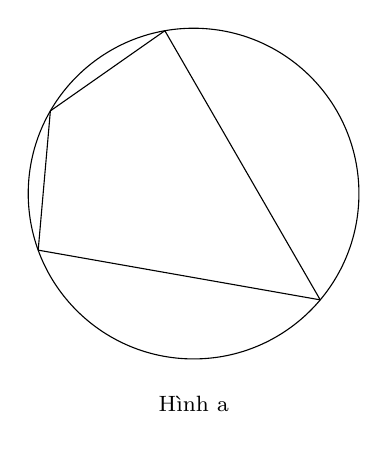
\begin{tikzpicture}[scale=0.7,>=stealth, font=\footnotesize, line join=round, line cap=round]
				\path 
				(-40:3) coordinate (A)
				(100:3) coordinate (B)
				(150:3) coordinate (C)
				(200:3) coordinate (D)
				;
				\draw (0,0) circle (3cm);
				\draw (A)--(B)--(C)--(D)--(A);
				\node at (0,-3.5)[below]{Hình a};
			\end{tikzpicture}
			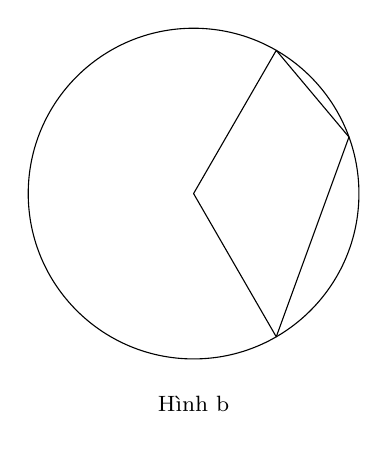
\begin{tikzpicture}[scale=0.7,>=stealth, font=\footnotesize, line join=round, line cap=round]
				\path 
				(0,0) coordinate (A)
				(60:3) coordinate (B)
				(20:3) coordinate (C)
				(-60:3) coordinate (D)
				;
				\draw (0,0) circle (3cm);
				\draw (A)--(B)--(C)--(D)--(A);
				\node at (0,-3.5)[below]{Hình b};
			\end{tikzpicture}
			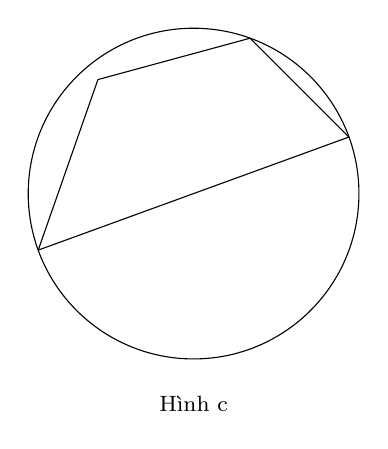
\begin{tikzpicture}[scale=0.7,>=stealth, font=\footnotesize, line join=round, line cap=round]
				\path 
				(20:3) coordinate (A)
				(70:3) coordinate (B)
				(130:2.7) coordinate (C)
				(200:3) coordinate (D)
				;
				\draw (0,0) circle (3cm);
				\draw (A)--(B)--(C)--(D)--(A);
				\node at (0,-3.5)[below]{Hình c};
			\end{tikzpicture}
			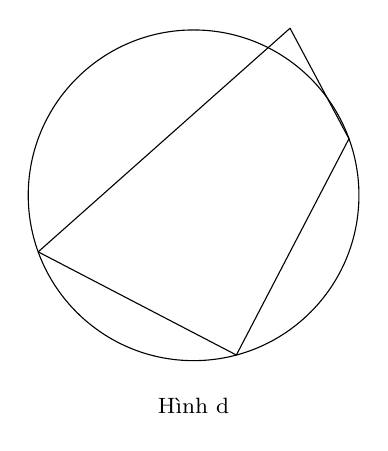
\begin{tikzpicture}[scale=0.7,>=stealth, font=\footnotesize, line join=round, line cap=round]
				\path 
				(20:3) coordinate (A)
				(60:3.5) coordinate (B)
				(200:3) coordinate (C)
				(-75:3) coordinate (D)
				;
				\draw (0,0) circle (3cm);
				\draw (A)--(B)--(C)--(D)--(A);
				\node at (0,-3.5)[below]{Hình d};
			\end{tikzpicture}
		\end{multicols}
	\end{center}
	\choice
	{\True Hình a}
	{Hình b}
	{Hình c}
	{Hình d}
	\loigiai{
		Dựa vào hình vẽ, ta thấy tứ giác ở hình a có bốn đỉnh nằm trên đường tròn nên tứ giác đó nội tiếp được đường tròn.
	}
\end{ex}

\begin{ex}%[Đề cương THCS]%[Nguyễn Văn Cường (Cường NV)]%[9H3N2-2] 
	Tứ giác $ABCD$ nội tiếp đường tròn biết $\widehat{BAD}=60^\circ$, số đó $\widehat{BCD}$ là bao nhiêu độ?
	\choice
	{$100^\circ$}
	{$40^\circ$}
	{$70^\circ$}
	{\True $120^\circ$}
	\loigiai{
		Vì tứ giác $ABCD$ nội tiếp đường tròn nên ta có $\widehat{BAD}+\widehat{BCD}=180^\circ$. \\
		Mà $\widehat{BAD}=60^\circ$ nên ta có $\widehat{BCD}=180^\circ-60^\circ=120^\circ$.	
	}
\end{ex}

\begin{ex}%[Đề cương THCS]%[Nguyễn Văn Cường (Cường NV)]%[9H3N3-1] 
	Trong các hình sau, hình nào \textbf{không} phải đa giác đều?
	\begin{center}
		\begin{multicols}{4}
			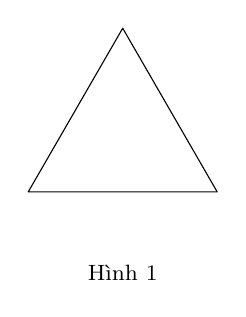
\begin{tikzpicture}[scale=0.8,>=stealth, font=\footnotesize, line join=round, line cap=round]
				\path 
				(0,0) coordinate (A)
				(0:3) coordinate (B)
				(60:3) coordinate (C)
				;
				\draw (A)--(B)--(C)--(A);
				\node at (1.5,-1)[below]{Hình 1};
			\end{tikzpicture}
			\begin{tikzpicture}[scale=0.8,>=stealth, font=\footnotesize, line join=round, line cap=round]
				\draw (0,0) rectangle (4,2);
				\node at (2,-1.6)[below]{Hình 2};
			\end{tikzpicture}
			\begin{tikzpicture}[scale=0.8,>=stealth, font=\footnotesize, line join=round, line cap=round]
				\draw (0,0) rectangle (3,3);
				\node at (1.5,-0.6)[below]{Hình 3};
			\end{tikzpicture}
			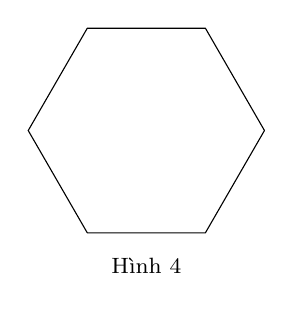
\begin{tikzpicture}[scale=0.6,>=stealth, font=\footnotesize, line join=round, line cap=round]
				\path 
				(0:2.5) coordinate (A)
				(60:2.5) coordinate (B)
				(120:2.5) coordinate (C)
				(180:2.5) coordinate (D)
				(240:2.5) coordinate (E)
				(300:2.5) coordinate (F)
				;
				\draw (A)--(B)--(C)--(D)--(E)--(F)--(A);
				\node at (0,-2.5)[below]{Hình 4};
			\end{tikzpicture}
		\end{multicols}
	\end{center}
	\choice
	{Hình 1}
	{\True Hình 2}
	{Hình 3}
	{Hình 4}
	\loigiai{
		Dựa vào hình đã cho, ta thấy Hình 2 là hình chữ nhật nên không phải đa giác đều.
	}
\end{ex}

\begin{ex}%[Đề cương THCS]%[Nguyễn Văn Cường (Cường NV)]%[9H3N3-2] 
	Cho hình vuông $ABCD$ có tâm $O$. Phép quay $90^\circ$ tâm $O$ cùng chiều kim đồng hồ biến điểm $B$ thành điểm nào?
	\begin{center}
		\begin{tikzpicture}[scale=0.8,>=stealth, font=\footnotesize, line join=round, line cap=round]
			\path 
			(0,0) coordinate (A)
			(4,0) coordinate (B)
			(4,-4) coordinate (C)
			(0,-4) coordinate (D)
			($(A)!0.5!(C)$) coordinate (O)
			;
			\draw (A)--(B)--(C)--(D)--(A)--(C) (D)--(B);
			\foreach \d/\g in{A/135,B/45,C/-45,D/-135,O/-90}
			\draw[fill=black](\d)circle(1pt)node[shift={(\g:0.35)}]{$\d$};
			\foreach \x/\y/\z in {A/O/B}{
				\path pic[draw,angle radius=5pt]{right angle= \x--\y--\z};}
		\end{tikzpicture}
	\end{center}
	\choice
	{Điểm $A$}
	{Điểm $B$}
	{\True Điểm $C$}
	{Điểm $D$}
	\loigiai{
		Phép quay tâm $O$, góc quay $90^\circ$ cùng chiều kim đồng hồ biến điểm $B$ thành điểm $C$.
	}
\end{ex}


\begin{ex}%[Đề cương THCS]%[Nguyễn Văn Cường (Cường NV)]%[9H3H1-2]
	Cho tam giác đều $ABC$ có đường cao $AH=9$ cm. Bán kính $r$ của đường tròn nội tiếp tam giác có độ dài là
	\choice
	{$6$ cm}
	{\True $3$ cm}
	{$4{,}5$ cm}
	{$\dfrac{3\sqrt{3}}{2}$ cm}
\loigiai{
\immini{
Ta có $\triangle ABC$ đều, có $AH$ là đường cao nên $AH$ đồng thời là đường trung tuyến.\\
Gọi $I$ là tâm đường tròn nội tiếp tam giác $ABC$ nên $I$ cũng là trọng tâm $\triangle ABC$.\\
Suy ra
\[r=IH=\dfrac{1}{3}AH=\dfrac{1}{3}\cdot 9=3\ (\text{cm}).\]
		}{
			\begin{tikzpicture}[>=stealth,line join=round,line cap=round,font=\footnotesize,scale=1]
				\def\r{4};
				\def\g{60};
				\path
				(0,0) coordinate (B)
				(0:\r) coordinate (C)
				(\g:\r) coordinate (A)
				($(B)!(A)!(C)$) coordinate (H)
				($(B)!1mm!(A)$) coordinate (a1)
				($(B)!1mm!(C)$) coordinate (a2)
				($(a1)!0.5!(a2)$) coordinate (b)
				(intersection of A--H and B--b) coordinate (I)
				($(A)!(I)!(C)$) coordinate (M)
				($(A)!(I)!(B)$) coordinate (N)
				;
				\draw (I) let \p1=($(I)-(H)$) in circle({veclen(\x1,\y1)})
				(A)--(B)--(C)--cycle (A)--(H) (B)--(I)--(C) (M)--(I)--(N)
				;
				\foreach \x/\g in {I/55,H/-90,B/-135,C/-45,A/90,M/30,N/150}\fill[black](\x) circle (1pt) +(\g:3mm) node {$\x$};
				\pic[draw,angle radius=3mm]{angle=B--A--H};
				\pic[draw,angle radius=4mm]{angle=H--A--C};
				\foreach \x/\y/\z in {I/H/C,I/M/A,I/N/A}{\draw pic[draw,angle radius=2mm]{right angle=\x--\y--\z};}
			\end{tikzpicture}
		}
	}
\end{ex}


\begin{ex}%[Đề cương THCS]%[Nguyễn Văn Cường (Cường NV)]%[9H3N3-2]
Cho tam giác vuông cân $ABC$ có $AB=AC=4$ cm. Bán kính $R$ của đường tròn ngoại tiếp tam giác có độ dài là
\choice
	{\True $2\sqrt{2}$ cm}
	{$\sqrt{2}$ cm}
	{$4\sqrt{2}$ cm}
	{$8\sqrt{2}$ cm}
	\loigiai{
\immini{
Gọi $O$ là trung điểm của $BC$, suy ra $O$ là tâm đường tròn ngoại tiếp tam giác $ABC$.\\
			Bán kính đường tròn ngoại tiếp tam giác $ABC$ là
			\allowdisplaybreaks
			\begin{eqnarray*}
				R&=&\dfrac{1}{2}BC=\dfrac{1}{2}\sqrt{AB^2+AC^2}\\
				&=&\dfrac{1}{2}\sqrt{4^2+4^2}\\
				&=&\dfrac{1}{2}\cdot 4\sqrt{2}\\
				&=&2\sqrt{2}\;(\text{cm}).
			\end{eqnarray*}
		}{
			\begin{tikzpicture}[>=stealth,line join=round,line cap=round,font=\footnotesize,scale=1]
				\def\r{3};
				\path
				(0,0) coordinate (A)
				(0:\r) coordinate (C)
				(90:\r) coordinate (B)
				($(B)!0.5!(C)$) coordinate (O)
				;
				\draw (O) let \p1=($(O)-(A)$) in circle({veclen(\x1,\y1)})
				(A)--(B)--(C)--cycle (A)--(O)node[midway,sloped,above]{$R$}
				;
				\foreach \x/\g in {B/100,C/-20,A/-135,O/40}\fill[black](\x) circle (1pt) +(\g:3mm) node {$\x$};
				\foreach \x/\y/\z in {B/A/C}{\draw pic[draw,angle radius=2mm]{right angle=\x--\y--\z};}
			\end{tikzpicture}
		}
	}
\end{ex}


\begin{ex}%[Đề cương THCS]%[Nguyễn Văn Cường (Cường NV)]%[9H3N2-1]
	Tứ giác ở hình nào dưới đây là tứ giác nội tiếp trong đường tròn $(O)$?
	\begin{center}
		\begin{tabular}{c c c c}
			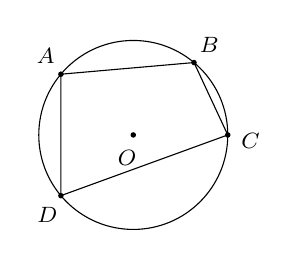
\begin{tikzpicture}[>=stealth,line join=round,line cap=round,font=\footnotesize,scale=1]
				\def\r{1.2};
				\path
				(0,0) coordinate (O)
				(140:\r) coordinate (A)
				(220:\r) coordinate (D)
				(360:\r) coordinate (C)
				(50:\r) coordinate (B)
				;
				\pgfresetboundingbox
				\draw (O) circle (\r)
				(A)--(B)--(C)--(D)--(A)
				;
				\foreach \x/\g in {A/130,O/-105,B/50,C/-15,D/-125}\fill[black](\x) circle (1pt) +(\g:3mm) node {$\x$};
			\end{tikzpicture} &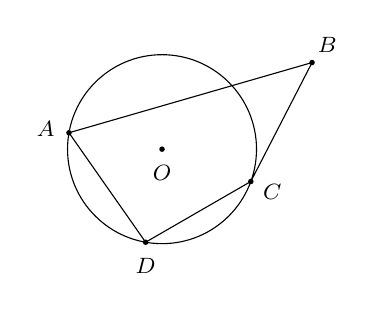
\begin{tikzpicture}[>=stealth,line join=round,line cap=round,font=\footnotesize,scale=1]
				\def\r{1.2};
				\path
				(0,0) coordinate (O)
				(170:\r) coordinate (A)
				(-100:\r) coordinate (D)
				(-20:\r) coordinate (C)
				(30:{\r+1}) coordinate (B)
				;
				\pgfresetboundingbox
				\draw (O) circle (\r)
				(A)--(B)--(C)--(D)--(A)
				;
				\foreach \x/\g in {A/170,O/-90,B/50,C/-25,D/-90}\fill[black](\x) circle (1pt) +(\g:3mm) node {$\x$};
			\end{tikzpicture} &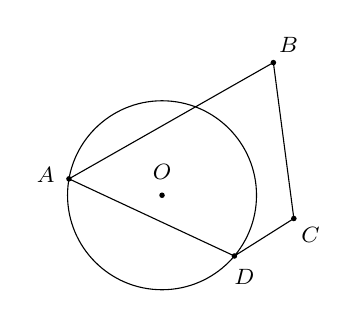
\begin{tikzpicture}[>=stealth,line join=round,line cap=round,font=\footnotesize,scale=1]
				\def\r{1.2};
				\path
				(0,0) coordinate (O)
				(170:\r) coordinate (A)
				(-40:\r) coordinate (D)
				(-10:{\r+0.5}) coordinate (C)
				(50:{\r+1}) coordinate (B)
				;
				\pgfresetboundingbox
				\draw (O) circle (\r)
				(A)--(B)--(C)--(D)--(A)
				;
				\foreach \x/\g in {A/170,O/90,B/50,C/-45,D/-65}\fill[black](\x) circle (1pt) +(\g:3mm) node {$\x$};
			\end{tikzpicture} &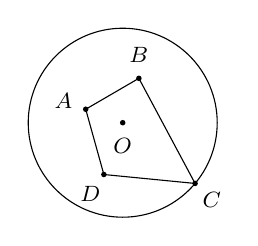
\begin{tikzpicture}[>=stealth,line join=round,line cap=round,font=\footnotesize,scale=1]
				\def\r{1.2};
				\path
				(0,0) coordinate (O)
				(160:{\r-0.7}) coordinate (A)
				(-110:{\r-0.5}) coordinate (D)
				(-40:\r) coordinate (C)
				(70:{\r-0.6}) coordinate (B)
				;
				\pgfresetboundingbox
				\draw (O) circle (\r)
				(A)--(B)--(C)--(D)--(A)
				;
				\foreach \x/\g in {A/160,O/-90,B/90,C/-45,D/-125}\fill[black](\x) circle (1pt) +(\g:3mm) node {$\x$};
			\end{tikzpicture}\\
			Hình 1 &Hình 2 &Hình 3 &Hình 4
		\end{tabular}
	\end{center}
	\choice
	{Hình 2}
	{Hình 3}
	{\True Hình 1}
	{Hình 4}
	\loigiai{
		Tứ giác $ABCD$ ở hình 1 là tứ giác nội tiếp.
	}
\end{ex}


\begin{ex}%[Đề cương THCS]%[Nguyễn Văn Cường (Cường NV)]%[9H3N2-1]
	Trong các phát biểu sau, phát biểu nào đúng?
	\choice
	{Mọi tứ giác luôn nội tiếp được đường tròn}
	{Trong một tứ giác nội tiếp, tổng số đo hai góc đối nhau bằng $90^\circ$}
	{\True Tổng số do hai góc đối của một tứ giác nội tiếp luôn bằng $180^\circ$}
	{Tất cả các hình thang đều là tứ giác nội tiếp}
	\loigiai{
		Khẳng định ``Tổng số do hai góc đối của một tứ giác nội tiếp luôn bằng $180^\circ$'' là đúng.
	}
\end{ex}


\begin{ex}%[Đề cương THCS]%[Nguyễn Văn Cường (Cường NV)]%[9H3H2-2]
	Cho tứ giác $MNPQ$ nội tiếp đường tròn $(O;R)$ và $\widehat{M}=60^\circ$. Số đo của $\widehat{P}$ là
	\choice
	{$30^\circ$}
	{\True $120^\circ$}
	{$180^\circ$}
	{$90^\circ$}
	\loigiai{
		\immini{
			Vì tứ giác $MNPQ$ nội tiếp đường tròn nên
			\allowdisplaybreaks
			\begin{eqnarray*}
				&&\widehat{M}+\widehat{P}=180^\circ\\
				&&\widehat{P}=180^\circ-\widehat{M}\\
				&&\widehat{P}=180^\circ-60^\circ=120^\circ.
			\end{eqnarray*}
		}{
			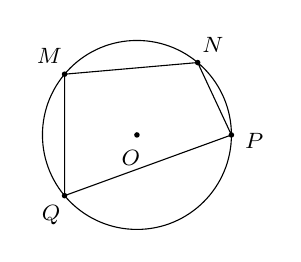
\begin{tikzpicture}[>=stealth,line join=round,line cap=round,font=\footnotesize,scale=1]
				\def\r{1.2};
				\path
				(0,0) coordinate (O)
				(140:\r) coordinate (M)
				(220:\r) coordinate (Q)
				(360:\r) coordinate (P)
				(50:\r) coordinate (N)
				;
				\pgfresetboundingbox
				\draw (O) circle (\r)
				(M)--(N)--(P)--(Q)--cycle
				;
				\foreach \x/\g in {M/130,O/-105,N/50,P/-15,Q/-125}\fill[black](\x) circle (1pt) +(\g:3mm) node {$\x$};
			\end{tikzpicture}
		}
	}
\end{ex}


\begin{ex}%[Đề cương THCS]%[Nguyễn Văn Cường (Cường NV)]%[9H3H2-2]
	\immini{
		Cho tứ giác $ABCD$ nội tiếp đường tròn $(O)$. Biết $\widehat{DAO}=50^\circ$, $\widehat{OCD}=30^\circ$ (Hình bên). Số đo của $\widehat{ABC}$ là
		\choice
		{$80^\circ$}
		{$90^\circ$}
		{\True $100^\circ$}
		{$110^\circ$}
	}{
		\begin{tikzpicture}[>=stealth,line join=round,line cap=round,font=\footnotesize,scale=1]
			\def\r{1.2};
			\path
			(0,0) coordinate (O)
			(140:\r) coordinate (A)
			(220:\r) coordinate (D)
			(360:\r) coordinate (C)
			(50:\r) coordinate (B)
			;
			\pgfresetboundingbox
			\draw (O) circle (\r)
			(C)--(O)--(A)--(B)--(C)--(D)--(A)
			;
			\foreach \x/\g in {A/130,O/-105,B/50,C/-15,D/-125}\fill[black](\x) circle (1pt) +(\g:3mm) node {$\x$};
			\pic[draw,angle radius=2mm]{angle=D--A--O};
			\pic[draw,angle radius=2mm,double]{angle=O--C--D};
			\node at ($(A)+(-60:0.5)$){\scriptsize $50^\circ$};
			\node at ($(C)+(190:0.7)$){\scriptsize $30^\circ$};
			%\path (current bounding box.south) node[below=2mm]{Hình 5};
		\end{tikzpicture}
	}
	\loigiai{
		\immini{
			Ta có $OA=OD=R$ nên $\triangle OAD$ cân tại $O$.\\
			Suy ra $\widehat{ODA}=\widehat{OAD}=50^\circ$.\hfill(1)\\
			Lại có $OC=OD=R$ nên $\triangle OCD$ cân tại $O$.\\
			Suy ra $\widehat{ODC}=\widehat{OCD}=30^\circ$.\hfill(2)\\
			Từ (1) và (2) suy ra $\widehat{ADC}= \widehat{ODA} + \widehat{ODC} =50^\circ+30^\circ=80^\circ$.\\
			Mà tứ giác $ABCD$ nội tiếp đường tròn nên
			\[\widehat{ABC}=180^\circ-\widehat{ADC}=180^\circ-80^\circ=100^\circ. \]
		}{
			\begin{tikzpicture}[>=stealth,line join=round,line cap=round,font=\footnotesize,scale=1]
				\def\r{2};
				\path
				(0,0) coordinate (O)
				(140:\r) coordinate (A)
				(220:\r) coordinate (D)
				(360:\r) coordinate (C)
				(50:\r) coordinate (B)
				;
				\pgfresetboundingbox
				\draw (O) circle (\r)
				(C)--(O)--(A)--(B)--(C)--(D)--(A) (O)--(D)
				;
				\foreach \x/\g in {A/130,O/-105,B/50,C/-15,D/-125}\fill[black](\x) circle (1pt) +(\g:3mm) node {$\x$};
				\pic[draw,angle radius=2mm]{angle=D--A--O};
				\pic[draw,angle radius=2mm,double]{angle=O--C--D};
				\node at ($(A)+(-60:0.5)$){\scriptsize $50^\circ$};
				\node at ($(C)+(190:0.7)$){\scriptsize $30^\circ$};
			\end{tikzpicture}
		}
	}
\end{ex}


\begin{ex}%[Đề cương THCS]%[Nguyễn Văn Cường (Cường NV)]%[9H3H2-2]
	Cho tứ giác $ABDC$ nội tiếp có $\widehat{ACD}=60^\circ$. Khẳng định nào sau đây luôn đúng?
	\choice
	{$\widehat{ADC}=60^\circ$}
	{$\widehat{ADC}=120^\circ$}
	{$\widehat{ABD}=60^\circ$}
	{\True $\widehat{ABD}=120^\circ$}
	\loigiai{
		\immini{
			Vì tứ giác $ABDC$ nội tiếp đường tròn nên
			\[\widehat{ACD}+\widehat{ABD}=180^\circ. \]
			Suy ra $\widehat{ABD}=180^\circ-\widehat{ACD}=180^\circ-60^\circ=120^\circ$.
		}{
			\begin{tikzpicture}[>=stealth,line join=round,line cap=round,font=\footnotesize,scale=1]
				\def\r{2};
				\path
				(0,0) coordinate (O)
				(100:\r) coordinate (A)
				(220:\r) coordinate (D)
				(10:\r) coordinate (C)
				(150:\r) coordinate (B)
				;
				\pgfresetboundingbox
				\draw (O) circle (\r)
				(A)--(B)--(D)--(C)--cycle (A)--(C)--(D)--cycle (B)--(C)
				;
				\foreach \x/\g in {A/130,O/-105,B/150,C/-15,D/-125}\fill[black](\x) circle (1pt) +(\g:3mm) node {$\x$};
				\pic[draw,angle radius=2mm]{angle=A--C--D};
				\node at ($(C)+(190:0.4)$){\scriptsize $60^\circ$};
			\end{tikzpicture}
		}
	}
\end{ex}


\begin{ex}%[Đề cương THCS]%[Nguyễn Văn Cường (Cường NV)]%[9H3H3-1]
	Cho lục giác đều $ABCDEF$ nội tiếp đường tròn bán kính $R$. Độ dài cạnh $AB$ bằng
	\choice
	{\True $R$}
	{$R\sqrt{3}$}
	{$\dfrac{R\sqrt{3}}{2}$}
	{$\dfrac{R}{2}$}
	\loigiai{
		\immini{
			Vì $ABCDEF$ là lục giác đều nên $\widehat{AOB}=60^\circ$.\\
			Mà $OA=OB=R$ nên tam giác $OAB$ đều.\\
			Do đó $AB=R$.
		}{
			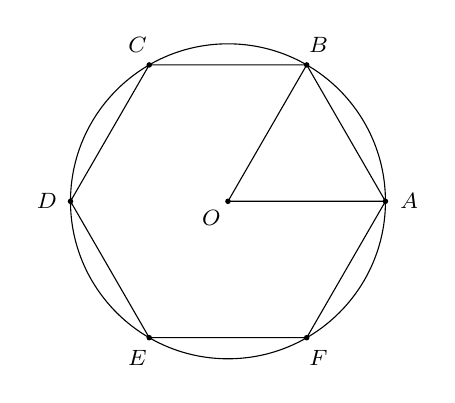
\begin{tikzpicture}[>=stealth,line join=round,line cap=round,font=\footnotesize,scale=1]
				\def\r{2};
				\path
				(0,0) coordinate (O)
				(0:\r) coordinate (A)
				(60:\r) coordinate (B)
				(120:\r) coordinate (C)
				(180:\r) coordinate (D)
				(240:\r) coordinate (E)
				(300:\r) coordinate (F)
				;
				\pgfresetboundingbox
				\draw (O) circle (\r)
				(A)--(B)--(C)--(D)--(E)--(F)--cycle (A)--(O)--(B)
				;
				\foreach \x/\g in {A/0,O/-135,B/60,C/120,D/180,E/240,F/300}\fill[black](\x) circle (1pt) +(\g:3mm) node {$\x$};
			\end{tikzpicture}
		}
	}
\end{ex}


\begin{ex}%[Đề cương THCS]%[Nguyễn Văn Cường (Cường NV)]%[9H3N3-2]
	Phép quay nào với $O$ là tâm biến tam giác đều thành chính nó?
	\choice
	{$90^\circ$}
	{$100^\circ$}
	{$110^\circ$}
	{\True $120^\circ$}
	\loigiai{
		\immini{
			Ba đỉnh $A$, $B$, $C$ của tam giác $ABC$ chia đường tròn $(O)$ thành ba cung bằng nhau, mỗi cung có số đo $360^\circ:3=120^\circ$. Từ đó các phép quay biến tam giác đều $ABC$ thành chính nó là các phép quay $120^\circ$, $240^\circ$ hoặc $360^\circ$ tâm $O$ cùng chiều kim đồng hồ hoặc ngược chiều kim đồng hồ.
		}{
			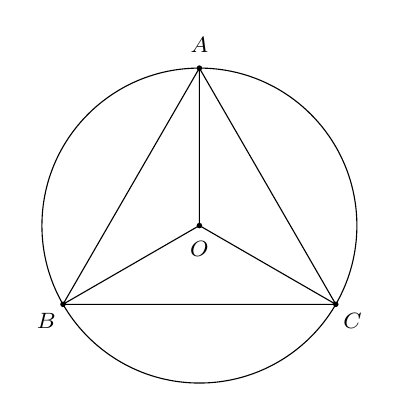
\begin{tikzpicture}[>=stealth,line join=round,line cap=round,font=\footnotesize,scale=1]
				\def\r{2};
				\path
				(0,0) coordinate (O)
				(90:\r) coordinate (A)
				(210:\r) coordinate (B)
				(330:\r) coordinate (C)
				;
				\draw (O) circle (\r)
				(A)--(B)--(C)--cycle (A)--(O)--(B) (O)--(C)
				;
				\foreach \x/\g in {B/-135,C/-45,A/90,O/-90}\fill[black](\x) circle (1pt) +(\g:3mm) node {$\x$};
			\end{tikzpicture}
		}
	}
\end{ex}

\subsection{Bài tập tự luận}

\begin{bt}%[Đề cương THCS]%[Nguyễn Văn Cường (Cường NV)]%[9H3N3-1]
	Quan sát các đa giác ở hình sau và cho biết đa giác nào là đa giác lồi.
	\begin{center}
		\begin{tabular}{cc}
			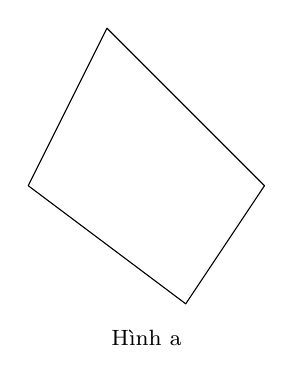
\begin{tikzpicture}[scale=1, font=\footnotesize, line join=round, line cap=round, >=stealth]
				\path (0,0) coordinate (A)
				(1,2) coordinate (B)
				(3,0) coordinate (C)
				(2,-1.5) coordinate (D);	
				\pgfresetboundingbox
				\draw (A)--(B)--(C)--(D)--(A);
				\path (current bounding box.south) node[below=2mm]{Hình a};
			\end{tikzpicture}
			\hspace*{2cm}
			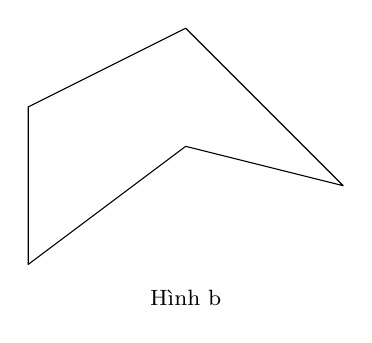
\begin{tikzpicture}[scale=1, font=\footnotesize, line join=round, line cap=round, >=stealth]
				\path (0,1) coordinate (A)
				(2,2) coordinate (B)
				(4,0) coordinate (C)
				(2,0.5) coordinate (D)
				(0,-1) coordinate (E);	
				\pgfresetboundingbox
				\draw (A)--(B)--(C)--(D)--(E)--(A);
				\path (current bounding box.south) node[below=2mm]{Hình b};
			\end{tikzpicture}
		\end{tabular}
	\end{center}	
	\loigiai{
		Hình $a$ là đa giác lồi.
	}
\end{bt}


\begin{bt}%[Đề cương THCS]%[Nguyễn Văn Cường (Cường NV)]%[9H3N3-1]
	Cho các vật thể có dạng đa giác đều như ở sau. Gọi tên từng đa giác đều đó.	
	\begin{center}
		\begin{tabular}{ccc}
			\begin{tikzpicture}%p  là số cạnh thì độ lớn của một góc (1-2\p)*180 và tổng số đo góc (p-2)*180
				\def\n{5}
				\pgfmathsetmacro{\goc}{(180-(1-2/\n)*180)}
				\foreach \x in {1,...,\n} \coordinate (A\x) at ($(0,0)+(90-\goc*\x:2)$);
				\draw[fill=green!50] (A1)--(A2)--(A3)--(A4)--(A5)--cycle;
				\draw ($(A3)!0.5!(A2)$) node[below]{$a$};
			\end{tikzpicture}
			\hspace*{2cm}
			\begin{tikzpicture}%p  là số cạnh thì độ lớn của một góc (1-2\p)*180 và tổng số đo góc (p-2)*180
				\def\n{6}
				\pgfmathsetmacro{\goc}{(180-(1-2/\n)*180)}
				\foreach \x in {1,...,\n} \coordinate (A\x) at ($(0,0)+(90-\goc*\x:2)$);
				\draw[fill=blue!30] (A1)--(A2)--(A3)--(A4)--(A5)--(A6)--cycle;
				\draw (A3) node[below]{$b$};
			\end{tikzpicture}
			\hspace*{2cm}
			\begin{tikzpicture}%p  là số cạnh thì độ lớn của một góc (1-2\p)*180 và tổng số đo góc (p-2)*180
				\def\n{8}
				\pgfmathsetmacro{\goc}{(180-(1-2/\n)*180)}
				\foreach \x in {1,...,\n} \coordinate (A\x) at ($(0,0)+(\goc*0.5-\goc*\x:2)$);
				\draw[fill=yellow!30] (A1)--(A2)--(A3)--(A4)--(A5)--(A6)--(A7)--(A8)--cycle;
				\draw ($(A3)!0.5!(A2)$) node[below]{$c$};
			\end{tikzpicture}
		\end{tabular}
	\end{center}
	\begin{center}
		\begin{tikzpicture}%p  là số cạnh thì độ lớn của một góc (1-2\p)*180 và tổng số đo góc (p-2)*180
			\def\n{9}
			\pgfmathsetmacro{\goc}{(180-(1-2/\n)*180)}
			\foreach \x in {1,...,\n} \coordinate (A\x) at ($(0,0)+(90-\goc*\x:2)$);
			\draw[fill=violet!10] (A1)--(A2)--(A3)--(A4)--(A5)--(A6)--(A7)--(A8)--(A9)--cycle;
			\draw ($(A4)!0.5!(A5)$) node[below]{$d$};
		\end{tikzpicture}
		\hspace*{2cm}
		\begin{tikzpicture}%p  là số cạnh thì độ lớn của một góc (1-2\p)*180 và tổng số đo góc (p-2)*180
			\def\n{10}
			\pgfmathsetmacro{\goc}{(180-(1-2/\n)*180)}
			\foreach \x in {1,...,\n} \coordinate (A\x) at ($(0,0)+(\goc*\x-\goc:2)$);
			\draw[fill=green!30] (A1)--(A2)--(A3)--(A4)--(A5)--(A6)--(A7)--(A8)--(A9)--(A10)--cycle;
			\draw ($(A9)!0.5!(A8)$) node[below]{$e$};
		\end{tikzpicture}
		\hspace*{2cm}
		\begin{tikzpicture}%p  là số cạnh thì độ lớn của một góc (1-2\p)*180 và tổng số đo góc (p-2)*180
			\def\n{12}
			\pgfmathsetmacro{\goc}{(180-(1-2/\n)*180)}
			\foreach \x in {1,...,\n} \coordinate (A\x) at ($(0,0)+(\goc*0.5-\goc*\x:2)$);
			\draw[fill=orange] (A1)--(A2)--(A3)--(A4)--(A5)--(A6)--(A7)--(A8)--(A9)--(A10)--(A11)--(A12)--cycle;
			\draw ($(A3)!0.5!(A4)$) node[below]{$f$};
		\end{tikzpicture}
	\end{center}
	\loigiai{
		\begin{enumerate}
			\item Ngũ giác đều.
			\item Lục giác đều.
			\item Bát giác đều.
			\item Cửu giác đều.
			\item Thập giác đều.
			\item Hình $12$ cạnh đều.
		\end{enumerate}		
	}
\end{bt}

%Bài 3
\begin{bt}%[Đề cương THCS]%[Nguyễn Văn Cường (Cường NV)]%[9H3N3-1]
	Mỗi phát biểu sau đây có đúng hay không? Vì sao?
	\begin{enumerate}
		\item Đa giác luôn nằm về một phía của đường thẳng chứa một cạnh bất kì của đa giác đó là đa giác lồi.
		\item Tứ giác có tất cả các cạnh bằng nhau là tứ giác đều.
		\item Tứ giác có tất cả các góc bằng nhau là tứ giác đều.
	\end{enumerate}	
	\loigiai{
		\begin{enumerate}
			\item ``Đa giác luôn nằm về một phía của đường thẳng chứa một cạnh bất kì của đa giác đó là đa giác lồi'' là phát biểu {\bf đúng}.
			\item ``Tứ giác có tất cả các cạnh bằng nhau là tứ giác đều'' là phát biểu {\bf sai}.
			\item ``Tứ giác có tất cả các góc bằng nhau là tứ giác đều'' là phát biểu {\bf sai}.
		\end{enumerate}		
	}
\end{bt}


\begin{bt}%[Đề cương THCS]%[Nguyễn Văn Cường (Cường NV)]%[9H3H3-1]
	Quan sát từng đa giác đều và tìm số thích hợp cho ``?'' trong bảng sau
	\begin{center}
		\begin{tabular}{|>{\centering\arraybackslash}p{2.5cm}|>{\centering\arraybackslash}p{2.5cm}|>{\centering\arraybackslash}p{2.5cm}|>{\centering\arraybackslash}p{4cm}|}
			\hline Đa giác đều & Số cạnh & Số góc & Số đo mỗi góc ( $\left.^{\circ}\right)$ \\
			\hline \begin{tikzpicture}[scale=.5, font=\footnotesize, line join=round, line cap=round, >=stealth]%p  là số cạnh thì độ lớn của một góc (1-2\p)*180 và tổng số đo góc (p-2)*180
				\def\n{6}
				\pgfmathsetmacro{\goc}{(180-(1-2/\n)*180)}
				\foreach \x in {1,...,\n} \coordinate (A\x) at ($(0,0)+(90-\goc*\x:2)$);
				\draw[fill=blue!10] (A1)--(A2)--(A3)--(A4)--(A5)--(A6)--cycle;
			\end{tikzpicture}& $?$ & $?$ & $?$ \\
			\hline \begin{tikzpicture}[scale=.5, font=\footnotesize, line join=round, line cap=round, >=stealth]%p  là số cạnh thì độ lớn của một góc (1-2\p)*180 và tổng số đo góc (p-2)*180
				\def\n{8}
				\pgfmathsetmacro{\goc}{(180-(1-2/\n)*180)}
				\foreach \x in {1,...,\n} \coordinate (A\x) at ($(0,0)+(90-\goc*\x:2)$);
				\draw[fill=green!20] (A1)--(A2)--(A3)--(A4)--(A5)--(A6)--(A7)--(A8)--cycle;
			\end{tikzpicture}& $?$ & $?$ & $?$ \\
			\hline
		\end{tabular}
	\end{center}	
	\loigiai{
		Ta có
		\begin{center}
			\begin{tabular}{|>{\centering\arraybackslash}p{2.5cm}|>{\centering\arraybackslash}p{2.5cm}|>{\centering\arraybackslash}p{2.5cm}|>{\centering\arraybackslash}p{4cm}|}
				\hline Đa giác đều & Số cạnh & Số góc & Số đo mỗi góc ( $\left.^{\circ}\right)$ \\
				\hline \begin{tikzpicture}[scale=.5, font=\footnotesize, line join=round, line cap=round, >=stealth]%p  là số cạnh thì độ lớn của một góc (1-2\p)*180 và tổng số đo góc (p-2)*180
					\def\n{6}
					\pgfmathsetmacro{\goc}{(180-(1-2/\n)*180)}
					\foreach \x in {1,...,\n} \coordinate (A\x) at ($(0,0)+(90-\goc*\x:2)$);
					\draw[fill=blue!10] (A1)--(A2)--(A3)--(A4)--(A5)--(A6)--cycle;
				\end{tikzpicture}& $6$ & $6$ & $120$ \\
				\hline \begin{tikzpicture}[scale=.5, font=\footnotesize, line join=round, line cap=round, >=stealth]%p  là số cạnh thì độ lớn của một góc (1-2\p)*180 và tổng số đo góc (p-2)*180
					\def\n{8}
					\pgfmathsetmacro{\goc}{(180-(1-2/\n)*180)}
					\foreach \x in {1,...,\n} \coordinate (A\x) at ($(0,0)+(90-\goc*\x:2)$);
					\draw[fill=green!20] (A1)--(A2)--(A3)--(A4)--(A5)--(A6)--(A7)--(A8)--cycle;
				\end{tikzpicture}& $8$ & $8$ & $135$ \\
				\hline
			\end{tabular}
		\end{center}		
		
	}
\end{bt}


\begin{bt}%[Đề cương THCS]%[Nguyễn Văn Cường (Cường NV)]%[9H3H3-1]
	Quan sát các hình sau và dùng compa, thước thẳng để vẽ lục giác đều theo cách đó.
	\begin{center}
		\begin{tabular}{ccc}
			\begin{tikzpicture}[scale = 0.7,transform shape]
				\tikzset{compa/.pic={
						\draw (2.95,3.7) rectangle (3,3.95);
						\draw (2.92,3.68) -- (2.5,2.5) -- (2.5,2.3) -- (2.99,3.68);
						\draw (3.5,2.5) -- (3.43,2.48);
						\draw (3.04,3.68) -- (3.5,2.5) -- (3.5,2.3) -- (2.975,3.68);
						\draw (2.5,2.5) -- (2.56,2.48);
						\draw[fill=white] (2.975,3.75) circle (0.1cm);
						\draw (2.975,3.75) circle (0.04cm);
						\draw (2.5,3.2) -- (3.5,3.2);
						\draw[line width = 0.5pt,line cap=round] (2.975,3.15) -- (2.975,3.25);}}
				\clip (-2.5,-3) rectangle + (5,5.5);
				\draw[red, line width = 2pt]
				($(0,0) + (30:2)$) arc (30:-220:2);
				
				\begin{scope}
					\path (-3.9,-3.9) pic[rotate = 20,scale =2,yscale = 0.5] {compa};
				\end{scope}
				\fill (0,0) circle (1pt);
				\draw (0,-2.5)node{$a)$};
			\end{tikzpicture}
			\hspace*{1.5cm}
			\begin{tikzpicture}[scale = 0.7,transform shape]
				\tikzset{compa/.pic={
						\draw (2.95,3.7) rectangle (3,3.95);
						\draw (2.92,3.68) -- (2.5,2.5) -- (2.5,2.3) -- (2.99,3.68);
						\draw (3.5,2.5) -- (3.43,2.48);
						\draw (3.04,3.68) -- (3.5,2.5) -- (3.5,2.3) -- (2.975,3.68);
						\draw (2.5,2.5) -- (2.56,2.48);
						\draw[fill=white] (2.975,3.75) circle (0.1cm);
						\draw (2.975,3.75) circle (0.04cm);
						\draw (2.5,3.2) -- (3.5,3.2);
						\draw[line width = 0.5pt,line cap=round] (2.975,3.15) -- (2.975,3.25);},
					gach/.pic={
						\draw[red,line width = 1pt] (0,0) arc (-10:10:1);}
				}
				\clip (-3,-3) rectangle + (5.5,5.5);
				\draw[red, line width = 2pt]
				(0,0) circle (2);
				\fill (0,0) circle (1pt);
				\path ($(0,0)+(0:1.8)$) pic[rotate = -80]{gach};
				\path ($(0,0)+(60:1.8)$) pic[rotate = -60]{gach};
				\path ($(0,0)+(120:1.8)$) pic[rotate = 40]{gach};
				\path ($(0,0)+(180:1.8)$) pic[rotate = 60]{gach};
				\path ($(0,0)+(240:1.8)$) pic[rotate=140]{gach};
				\path ($(0,0)+(300:1.8)$) pic[rotate=200]{gach};
				\draw[dashed,line width = 1pt, green] (0,0)--++(238:2)--($(0,0)+(177:2)$);
				\begin{scope}
					\path (3.1,-5.3) pic[rotate = 115,scale =2,yscale = 0.5] {compa};
				\end{scope}
				\draw (0,-2.5)node{$b)$};
			\end{tikzpicture}
			\hspace*{1.5cm}
			\begin{tikzpicture}[scale = 0.7,transform shape]
				\tikzset{compa/.pic={
						\draw (2.95,3.7) rectangle (3,3.95);
						\draw (2.92,3.68) -- (2.5,2.5) -- (2.5,2.3) -- (2.99,3.68);
						\draw (3.5,2.5) -- (3.43,2.48);
						\draw (3.04,3.68) -- (3.5,2.5) -- (3.5,2.3) -- (2.975,3.68);
						\draw (2.5,2.5) -- (2.56,2.48);
						\draw[fill=white] (2.975,3.75) circle (0.1cm);
						\draw (2.975,3.75) circle (0.04cm);
						\draw (2.5,3.2) -- (3.5,3.2);
						\draw[line width = 0.5pt,line cap=round] (2.975,3.15) -- (2.975,3.25);},
					gach/.pic={
						\draw[red,line width = 1pt] (0,0) arc (-10:10:1);},
					ruler/.pic={
						\draw (-0.001,0) rectangle (5,0.5);
						\foreach \x in {1,...,10} \draw[line width=1pt] (\x*0.5,0.5)--(\x*0.5,0.4) node[below]{\tiny$\x$};
					},
					pencil/.pic={
						\fill[gray!50] (0,4) -- (0.4,4) -- (0.4,0) --(0.3,-0.15) -- (0.2,0) -- (0.1,-0.14) -- (0,0) -- cycle;
						\draw[color=white] (0.2,4) -- (0.2,0);
						\fill[black] (0,3.5) -- (0.2,3.47) -- (0.4,3.5) -- (0.4,4) arc(30:150:0.23cm);
						\fill[brown!40] (0,0) -- (0.2,-0.8)node[coordinate,pos=0.75](a){} -- (0.4,0)node[coordinate,pos=0.25](b){} -- (0.3,-0.15) -- (0.2,0) -- (0.1,-0.14) -- cycle;
						\fill[gray] (a) -- (0.2,-0.8) -- (b) -- cycle;
					}
				}
				\clip (-3,-3) rectangle + (5.5,5.5);
				\draw[red, line width = 2pt]
				(0,0) circle (2);
				\fill (0,0) circle (1pt);
				\path ($(0,0)+(0:1.8)$) pic[rotate = -80]{gach};
				\path ($(0,0)+(60:1.8)$) pic[rotate = -60]{gach};
				\path ($(0,0)+(120:1.8)$) pic[rotate = 40]{gach};
				\path ($(0,0)+(180:1.8)$) pic[rotate = 60]{gach};
				\path ($(0,0)+(240:1.8)$) pic[rotate=140]{gach};
				\path ($(0,0)+(300:1.8)$) pic[rotate=200]{gach};
				\foreach \x in {1,2,...,6} \coordinate (A\x) at ($(0,0)+(60*\x:2)$);
				\draw[line width=1pt, green!50!black] (A1)--(A2)--(A3)--(A4)--(A5)--(A6);
				\draw (0,-2.5)node{$c)$};
				\path (0.3,2)pic[rotate = -60]{ruler};
				\path (1.6,1.5) pic[rotate = -30,scale = 0.8]{pencil};
			\end{tikzpicture}
		\end{tabular}
	\end{center}
	\loigiai{Dùng compa và thước thẳng ta vẽ được hình lục giác đều sau.
		\begin{center}
			\begin{tikzpicture}[scale=1, font=\footnotesize, line join=round, line cap=round, >=stealth]%p  là số cạnh thì độ lớn của một góc (1-2\p)*180 và tổng số đo góc (p-2)*180
				\def\n{6}
				\pgfmathsetmacro{\goc}{(180-(1-2/\n)*180)}
				\foreach \x in {1,...,\n} \coordinate (A\x) at ($(0,0)+(90-\goc*\x:2)$);
				\draw[fill=cyan!20] (A1)--(A2)--(A3)--(A4)--(A5)--(A6)--cycle;
			\end{tikzpicture}
	\end{center}}
\end{bt}

\begin{bt}%[Đề cương THCS]%[Nguyễn Văn Cường (Cường NV)]%[9H3H3-2]
	Hãy tìm hiểu và chỉ ra những vật thể trong thực tiễn mà cấu trúc của nó có dạng hình đa giác đều.	
	\loigiai{
		Những vật thể trong thực tiễn mà cấu trúc của nó có dạng hình đa giác đều là
		\begin{itemize}
			\item Viên gạch men lát nền nhà.
			\item Gạch hình lục giác lát vỉa hè.
			\item Biển báo hình tam giác.
		\end{itemize}	
	}
\end{bt}

\begin{bt}%[Đề cương THCS]%[Nguyễn Văn Cường (Cường NV)]%[9H3H3-1]
	Cho một hình lục giác đều và một hình vuông cùng nội tiếp một đường tròn. Biết rằng hình vuông có cạnh bằng $3$ cm. Tính chu vi và diện tích của một hình lục giác đều đã cho.
	\loigiai{
		\immini{
			Xét hình vuông $MNPQ$ nội tiếp đường tròn $O$, có $O$ cũng là giao điểm của hai đường chéo.\\
			Do đó, bán kính đường tròn ngoại tiếp là
			\[R=\dfrac{MP}{2}=\dfrac{\sqrt{MN^2+NP^2}}{2}=\dfrac{\sqrt{3^2+3^2}}{2}=\dfrac{3\sqrt{2}}{2}\;(\text{cm}).\]
			Xét tam giác $COD$ cân tại $O$, có $\widehat{COD}=\dfrac{360^\circ}{6}=60^\circ$ nên là tam giác đều.
		}{
			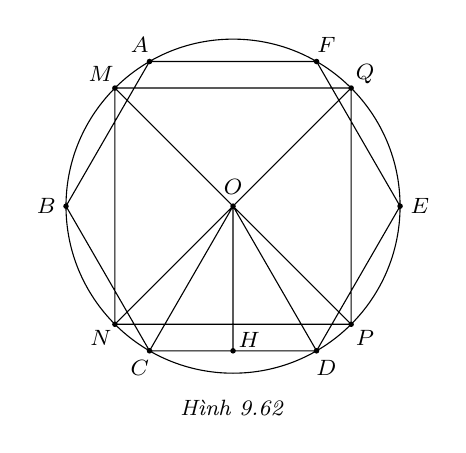
\begin{tikzpicture}[font=\footnotesize,scale=1,declare function={a=3;b=a*sin 45;}]
				\path 
				(0,0) coordinate (O) (135:b) coordinate (M) (-135:b) coordinate (N) (-45:b) coordinate (P) (45:b) coordinate (Q)
				(120:b) coordinate (A) (180:b) coordinate (B) (-120:b) coordinate (C) (-60:b) coordinate (D) (0:b) coordinate (E) (60:b) coordinate (F) (-90:{b*sin 60}) coordinate (H);
				\draw (O) circle (b) (M)--(N)--(P)--(Q)--cycle (A)--(B)--(C)--(D)--(E)--(F)--cycle
				(C)--(O)--(D) (N)--(Q) (M)--(P) (O)--(H);
				\foreach \i/\j in {M/135,N/-135,P/-45,O/90,Q/45,A/120,B/180,C/-120,D/-60,E/0,F/60,H/35}
				\fill (\i) circle (1pt) (\i)node[shift={(\j:2.5mm)}]{$\i$};
				\path (current bounding box.south) node[below=2pt]{\textit{Hình 9.62}};
			\end{tikzpicture}	
		}
		\noindent
		Suy ra $CD=R=\dfrac{3\sqrt{2}}{2}$ (cm).\\
		Chu vi của lục giác đều $ABCDEF$ là $6CD=9\sqrt{2}$ (cm).\\
		Diện tích của lục giác đều $ABCDEF$ là 
		\[6S_{OCD}=6\cdot \dfrac{1}{2} \cdot CD \cdot OH=3 \cdot R \cdot R \cdot \sin 60^\circ=\dfrac{27\sqrt{3}}{4}\; (\text{cm}^2).\]
	}
\end{bt}

\begin{bt}%[Đề cương THCS]%[Nguyễn Văn Cường (Cường NV)]%[9H3N3-2]
	\immini{
		Cho hình vuông $ABCD$ có tâm $O$ (Hình bên). Phép quay thuận chiều tâm $O$ biến điểm $A$ thành điểm $D$ thì các điểm $B, C, D$ tương ứng biến thành các điểm nào?
	}{
		\begin{tikzpicture}[scale=1, font=\footnotesize,>=stealth, thick]
			%Gán số liệu.
			\def\canhAD{3};
			%Gán tọa độ.
			\coordinate (D) at (0,0);
			\coordinate (A) at ($(D)+(90:\canhAD)$);
			\coordinate (C) at ($(D)+(0:\canhAD)$);
			\coordinate (B) at ($(A)+(0:\canhAD)$);
			\coordinate (O) at (intersection of A--C and B--D);
			%Vẽ hình vuông ADCB.
			\draw (A) rectangle (C);
			\draw[dashed](A)--(C)(B)--(D);
			%Gán nhãn.
			\foreach \x/\y in {A/90,D/-90,C/-90,B/90, O/-90}{\fill (\x) circle(1pt) ($(\x)+(\y:0.3cm)$) node{$\x$};}
		\end{tikzpicture}
	}
	\loigiai
	{
		Phép quay thuận chiều tâm $O$ biến điểm $A$ thành điểm $D$ thì các điểm $B$, $C$, $D$ tương ứng biến thành các điểm $A$, $B$, $C$.
	}
\end{bt}


\begin{bt}%[Đề cương THCS]%[Nguyễn Văn Cường (Cường NV)]%[9H3H3-2]
	\hfill
	\immini{
		\begin{listEX}[1]
			\item Phép quay thuận chiều $45^{\circ}$ tâm $O$ biến các điểm $A$, $B$, $C$, $D$ lần lượt thành các điểm  $A^{'}$, $B^{'}$, $C^{'}$, $D^{'}$ (Hình bên). Hãy vẽ tứ giác $A^{'}B^{'}C^{'}D^{'}$.
			\item Phép quay trong câu a biến các điểm $A^{'}$, $B^{'}$, $C^{'}$, $D^{'}$ thành những điểm nào?
		\end{listEX}
	}{
		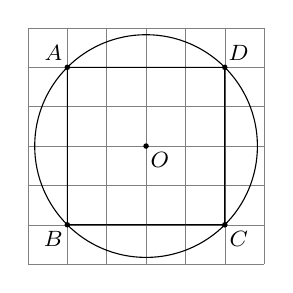
\begin{tikzpicture}[font=\footnotesize,scale=1,declare function={a=2;b=a*sin 45;}]
			\draw[step=0.5,gray,very thin] (-1.5,-1.5) grid (1.5,1.5);
			\path (0,0) coordinate (O) (135:b) coordinate (A) (-135:b) coordinate (B) (-45:b) coordinate (C) (45:b) coordinate (D);
			\draw (O) circle (b) (B) rectangle (D);
			\foreach \i/\j in {A/135,B/-135,C/-45,O/-45,D/45}\fill (\i) circle (1pt) (\i)node[shift={(\j:2.5mm)}]{$\i$};
		\end{tikzpicture}
	}
	\loigiai{
		\immini{
			\begin{listEX}[1]
				\item Phép quay thuận chiều $45^{\circ}$ tâm $O$ biến các điểm $A$, $B$, $C$, $D$ lần lượt thành các điểm  $A'$, $B'$, $C'$, $D^{'}$. Tứ giác $A^{'}B^{'}C^{'}D^{'}$ như hình bên.
				\item Phép quay trong câu a biến các điểm $A'$, $B'$, $C'$, $D'$ lần lượt thành $D$, $A$, $B$, $C$.
			\end{listEX}
		}{
			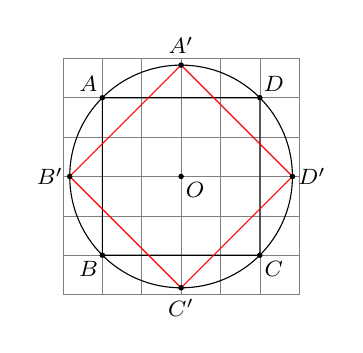
\begin{tikzpicture}[font=\footnotesize,scale=1,declare function={a=2;b=a*sin 45;}]
				\draw[step=0.5,gray,very thin] (-1.5,-1.5) grid (1.5,1.5);
				\path 
				(0,0) coordinate (O) (135:b) coordinate (A) (-135:b) coordinate (B) (-45:b) coordinate (C) (45:b) coordinate (D)
				(90:b) coordinate (A') (180:b) coordinate (B') (-90:b) coordinate (C') (0:b) coordinate (D');
				\draw (O) circle (b) (B) rectangle (D);
				\draw[red] (90:b) --(0:b)--(-90:b)--(180:b)--cycle;
				\foreach \i/\j in {A/135,B/-135,C/-45,O/-45,D/45,A'/90,B'/-180,C'/-90,D'/0}
				\fill (\i) circle (1pt) (\i)node[shift={(\j:2.5mm)}]{$\i$};
			\end{tikzpicture}
		}
	}
\end{bt}

\begin{bt}%[Đề cương THCS]%[Nguyễn Văn Cường (Cường NV)]%[9H3H3-2]
	~
	\begin{enumerate}
		\item Ở Hình $a$, ta thực hiện phép quay ngược chiều giữ nguyên hình đa giác đều $ABCDEGH$ (có $7$ cạnh) và biến các điểm $A$; $B$; $C$; $D$; $E$; $G$; $H$ lần lượt thành các điểm $H$; $A$; $B$; $C$; $D$; $E$; $G$. Phép quay đó là phép quay nào?
		\item Ở Hình $b$, ta thực hiện phép quay thuận chiều giữ nguyên hình đa giác đều $ABCDEGH$ (có $7$ cạnh) và biến các điểm $A$; $B$; $C$; $D$; $E$; $G$; $H$ lần lượt thành các điểm $B$; $C$; $D$; $E$; $G$; $H$; $A$. Phép quay đó là phép quay nào?
		\begin{center}
			\begin{tabular}{cc}
				\begin{tikzpicture}[shorten <=5pt,shorten >=5pt]%p  là số cạnh thì độ lớn của một góc (1-2\p)*180 và tổng số đo góc (p-2)*180
					\def\n{7}
					\pgfmathsetmacro{\goc}{(180-(1-2/\n)*180)}
					\foreach \x in {1,...,\n} \coordinate (A\x) at ($(0,0)+(90-\goc*\x:2)$);
					\draw[blue,line width = 1pt] (A1)--(A2)--(A3)--(A4)--(A5)--(A6)--(A7)--cycle;
					\foreach \x/\y in {1/B,2/C,3/D,4/E,5/G,6/H,7/A}{\coordinate (\y) at ($(0,0)+(90-\goc*\x:2.2)$); 
						\draw (\y) node{$\y$};}
					\path [-stealth,red] (C) edge node {} (B);
					\path [-stealth,red] (B) edge node {} (A);
					\path[-stealth,red] (A) edge node {} (H);
					\draw (0,-2.5) node {$a)$};
				\end{tikzpicture}
				\hspace*{2cm}
				\begin{tikzpicture}[shorten <=5pt,shorten >=5pt]%p  là số cạnh thì độ lớn của một góc (1-2\p)*180 và tổng số đo góc (p-2)*180
					\def\n{7}
					\pgfmathsetmacro{\goc}{(180-(1-2/\n)*180)}
					\foreach \x in {1,...,\n} \coordinate (A\x) at ($(0,0)+(90-\goc*\x:2)$);
					\draw[blue,line width = 1pt] (A1)--(A2)--(A3)--(A4)--(A5)--(A6)--(A7)--cycle;
					\foreach \x/\y in {1/B,2/C,3/D,4/E,5/G,6/H,7/A}{\coordinate (\y) at ($(0,0)+(90-\goc*\x:2.2)$); 
						\draw (\y) node{$\y$};}
					\path [-stealth,red] (A) edge node {} (B);
					\path [-stealth,red] (C) edge node {} (D);
					\path[-stealth,red] (B) edge node {} (C);
					\draw (0,-2.5) node {$b)$};
				\end{tikzpicture}
			\end{tabular}
		\end{center}
		\item Ở Hình $c$, ta thực hiện phép quay thuận chiều giữ nguyên hình đa giác đều $ABCDEGHK$ (có 8 cạnh) và biến các điểm $A$, $B$, $C$, $D$, $E$, $G$, $H$, $K$ lần lượt thành các điểm $B$, $C$, $D$, $E$, $G$, $H$, $K$, $A$. Phép quay đó là phép quay nào?
		\item Ở Hình $d$, ta thực hiện phép quay ngược chiều giữ nguyên hình đa giác đều $ABCDEGHK$ (có 8 cạnh) và biến các điểm $A$, $B$, $C$, $D$, $E$, $G$, $H$, $K$ lần lượt thành các điểm $K$, $A$, $B$, $C$, $D$, $E$, $G$, $H$. Phép quay đó là phép quay nào?
		\begin{center}
			\begin{tabular}{cc}
				\begin{tikzpicture}[shorten <=5pt,shorten >=5pt]%p  là số cạnh thì độ lớn của một góc (1-2\p)*180 và tổng số đo góc (p-2)*180
					\def\n{8}
					\pgfmathsetmacro{\goc}{(180-(1-2/\n)*180)}
					\foreach \x in {1,...,\n} \coordinate (A\x) at ($(0,0)+(90-\goc*\x:2)$);
					\draw[blue,line width = 1pt] (A1)--(A2)--(A3)--(A4)--(A5)--(A6)--(A7)-- (A8)--cycle;
					\foreach \x/\y in {8/B,1/C,2/D,3/E,4/G,5/H,6/K,7/A}{\coordinate (\y) at ($(0,0)+(90-\goc*\x:2.2)$); 
						\draw (\y) node{$\y$};}
					\path [-stealth,red] (A) edge node {} (B);
					\path [-stealth,red] (B) edge node {} (C);
					\path[-stealth,red] (C) edge node {} (D);
					\draw (0,-2.8) node {$c)$};
				\end{tikzpicture}
				\hspace*{2cm}
				\begin{tikzpicture}[shorten <=5pt,shorten >=5pt]%p  là số cạnh thì độ lớn của một góc (1-2\p)*180 và tổng số đo góc (p-2)*180
					\def\n{8}
					\pgfmathsetmacro{\goc}{(180-(1-2/\n)*180)}
					\foreach \x in {1,...,\n} \coordinate (A\x) at ($(0,0)+(90-\goc*\x:2)$);
					\draw[blue,line width = 1pt] (A1)--(A2)--(A3)--(A4)--(A5)--(A6)--(A7)--(A8)--cycle;
					\foreach \x/\y in {1/C,2/D,3/E,4/G,5/H,6/K,7/A,8/B}{\coordinate (\y) at ($(0,0)+(90-\goc*\x:2.2)$); 
						\draw (\y) node{$\y$};}
					\path [-stealth,red] (C) edge node {} (B);
					\path [-stealth,red] (B) edge node {} (A);
					\path[-stealth,red] (A) edge node {} (K);
					\draw (0,-2.8) node {$d)$};
				\end{tikzpicture}
			\end{tabular}
		\end{center}
	\end{enumerate}	
	\loigiai{
		Gọi $O$ là tâm của hình lục giác đều $ABCDEGHK$.
		\begin{enumerate}
			\item Ở hình $a$ thực hiện phép quay ngược chiều $\alpha^\circ$ tâm $O$ với $\alpha^\circ = \dfrac{360^\circ}{7}$.
			\item Ở hình $b$ thực hiện phép quay thuận chiều $\alpha^\circ$ tâm $O$ với $\alpha^\circ = \dfrac{360^\circ}{7}$.
			\item Ở hình $c$ thực hiện phép quay thuận chiều $\alpha^\circ$ tâm $O$ với $\alpha^\circ = \dfrac{360^\circ}{8} = 45^\circ$.
			\item Ở hình $d$ thực hiện phép quay ngược chiều $\alpha^\circ$ tâm $O$ với $\alpha^\circ = \dfrac{360^\circ}{8} = 45^\circ$.
		\end{enumerate}
	}
\end{bt}

\begin{bt}%[Đề cương THCS]%[Nguyễn Văn Cường]%[9H3H3-1]%[9H3V3-2]
	\immini{
		Mái nhà trong hình bên được đỡ bởi khung hình đa giác đều. Gọi tên đa giác đó và tìm phép quay biến đa giác đó thành chính nó.
	}{
		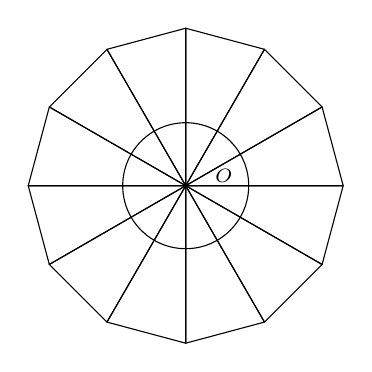
\begin{tikzpicture}[>=stealth,line join=round,line cap=round,font=\footnotesize,scale=1]
			\def\r{2};
			%\foreach \x/\p in {0/A,30/B,60/C,90/D,120/E,150/F,180/G,210/H,240/I,270/J,300/K,330/L}{\path (\x:\r) coordinate ($\p$);
				%\node at ($(\x:\r)+(\x:0.3)$){$\p$};}
			\foreach \g in {0,30,...,330}{\draw (\g:\r)--(\g+30:\r)--(\g+210:\r);}
			\draw (0,0) circle (0.8);
			\node at (15:0.5){\scriptsize $O$};
		\end{tikzpicture}
	}
	\loigiai
	{
		Đa giác đều $12$ cạnh gọi là thập nhị giác đều.\\
		Ta có $12$ đỉnh của đa giác chia đường tròn thành $12$ phần bằng nhau nên số đo mỗi cung là $360^\circ:12=30^\circ$.\\
		Gọi $O$ là tâm đường tròn ngoại tiếp của tam giác đều $12$ cạnh.\\
		Phép quay $30^\circ$, $60^\circ$, $90^\circ$,$\ldots$, $360^\circ$ tâm $O$ cùng hoặc ngược chiều kim đồng hồ biến đa giác đều $12$ cạnh thành chính nó.	
	}
\end{bt} 


\begin{bt}%[Đề cương THCS]%[Nguyễn Văn Cường (Cường NV)]%[9H3H2-2]
\immini{Cho tam giác nhọn $ABC$ có đường cao $AH$ ($H \in BC$) và nội tiếp đường tròn tâm $O$ có đường kính $AM$ (Hình bên). Chứng minh $\widehat{OAC} = \widehat{BAH}$.
	}{
		\begin{tikzpicture}[>=stealth,line join=round,line cap=round,font=\footnotesize,scale=1]
			\def\r{2};
			\path
			(0,0) coordinate (O)
			(180:\r) coordinate (A)
			(0:\r) coordinate (M)
			(-50:\r) coordinate (B)
			(30:\r) coordinate (C)
			($(B)!(A)!(C)$) coordinate (H)
			;
			\draw (O) circle (\r)
			(H)--(A)--(B)--(C)--(A)--(M) (O)--(C)
			;
			\foreach \x/\g in {B/-50,C/30,A/180,O/140,H/-50,M/0}\fill[black](\x) circle (1pt) +(\g:3mm) node {$\x$};
			\pic[draw,angle radius=2mm]{right angle=A--H--B};
			%\path (current bounding box.south) node[below=2mm]{Hình 6};
		\end{tikzpicture}
	}
\loigiai{
\immini{
Xét đường tròn $(O)$ có $\widehat{ACM}=90^\circ$ (góc nội tiếp chắn nửa đường tròn).\\
Xét $\triangle ABH$ và $\triangle AMC$ có
\begin{itemize}
\item $\widehat{AHB}=\widehat{ACM}=90^\circ$.
\item $\widehat{AMC}=\widehat{ABH}$ ($2$ góc nội tiếp cùng chắn $\wideparen{AC}$).
\end{itemize}	
Suy ra $\triangle ABH\backsim\triangle AMC$ (g - g).\\
Do đó $\widehat{MAC}=\widehat{BAH}$ ($2$ góc tương ứng).\\
Hay $\widehat{OAC}=\widehat{BAH}$.
		}{
			\begin{tikzpicture}[>=stealth,line join=round,line cap=round,font=\footnotesize,scale=1]
				\def\r{2.5};
				\path
				(0,0) coordinate (O)
				(180:\r) coordinate (A)
				(0:\r) coordinate (M)
				(-50:\r) coordinate (B)
				(30:\r) coordinate (C)
				($(B)!(A)!(C)$) coordinate (H)
				;
				\draw (O) circle (\r)
				(H)--(A)--(B)--(C)--(A)--(M) (O)--(C)--(M)
				;
				\foreach \x/\g in {B/-50,C/30,A/180,O/140,H/-50,M/0}\fill[black](\x) circle (1pt) +(\g:3mm) node {$\x$};
			\foreach \x/\y/\z in {A/H/B,A/C/M}\pic[draw,angle radius=2.5mm]{right angle=\x--\y--\z};
			\end{tikzpicture}
		}
	}
\end{bt}


\begin{bt}%[Đề cương THCS]%[Nguyễn Văn Cường (Cường NV)]%[9H3V4-8]
	Cho tam giác $ABC$ vuông tại $A$ ($AB < AC$) có $AH$ là đường cao. Lần lượt vẽ đường tròn $(O)$ đường kính $BH$ và đường tròn $(O')$ đường kính $HC$.
	\begin{enumerate}
		\item Xét vị trí tương đối của đường tròn $(O)$ và $(O')$.
		\item Đường tròn $(O)$ cắt $AB$ tại $E$, đường tròn $(O')$ cắt $AC$ tại $F$. Chứng minh rằng tứ giác $AEHF$ là hình chữ nhật.
		\item Chứng minh rằng $EF$ là tiếp tuyến của đường tròn $(O)$ và đồng thời là tiếp tuyến của đường tròn $(O')$.
		\item Đường trung tuyến $AM$ của tam giác $ABC$ cắt $EF$ tại $N$. Cho biết $AB=6$ cm, $AC=8$ cm. Tính diện tích tam giác $ANF$.
	\end{enumerate}
	\loigiai{
		\immini{
			\begin{enumerate}
				\item Vì đường nối tâm $OO'=OH+HO'$ và $H\in OO'$ nên $(O)$ và $(O')$ tiếp xúc nhau.
				\item Ta có $\widehat{HEB}=\widehat{HFC}=90^\circ$ (góc nội tiếp chắn nửa đường tròn).\\
				Suy ra $HE\perp AB$ tại $E$ và $HF\perp CF$ tại $F$.\\
				Suy ra $\widehat{HEA}=\widehat{HFA}=90^\circ$.\\
				Tứ giác $AEHF$ có $\widehat{HEA}=\widehat{HFA}=\widehat{EAF}=90^\circ$.\\
				Suy ra $AEHF$ là hình chữ nhật.
			\end{enumerate}
		}{
			\begin{tikzpicture}[>=stealth,line join=round,line cap=round,font=\footnotesize,scale=1]
				\path
				(0,0) coordinate (A)
				(0,4) coordinate (B)
				(6,0) coordinate (C)
				($(B)!(A)!(C)$) coordinate (H)
				($(B)!0.5!(H)$) coordinate (O)
				($(C)!0.5!(H)$) coordinate (O')
				($(B)!0.5!(C)$) coordinate (M)
				;
				\path[name path=c1] (O) let \p1=($(O)-(H)$) in circle({veclen(\x1,\y1)});
				\path[name path=c2] (O') let \p1=($(O')-(H)$) in circle({veclen(\x1,\y1)});
				\path[name path=ab] (A)--(B);
				\path[name path=ac] (A)--(C);
				\path
				[name intersections={of=c1 and ab}] coordinate (E) at (intersection-2)
				[name intersections={of=c2 and ac}] coordinate (F) at (intersection-1)
				(intersection of E--F and A--M) coordinate (N)
				;
				\pgfresetboundingbox
				\draw (O) let \p1=($(O)-(H)$) in circle({veclen(\x1,\y1)})
				(O') let \p1=($(O')-(H)$) in circle({veclen(\x1,\y1)})
				(A)--(B)--(C)--cycle (A)--(H) (E)--(H)--(F)--cycle (O)--(E) (O')--(F) (A)--(M)--(F)
				;
				\foreach \x/\g in {A/-135,B/90,C/0,E/180,F/-90,H/-5,O/30,O'/30,M/40,N/-95}\fill[black](\x) circle (1pt) +(\g:3mm) node {$\x$};
				\pic[draw,angle radius=2mm]{right angle=C--A--B};
				\pic[draw,angle radius=2mm]{right angle=A--H--B};
			\end{tikzpicture}
		}
		\begin{enumerate}
			\setcounter{enumi}{2}
			\item Vì tứ giác $AEHF$ là hình chữ nhật nên $HE = AF$.\\
			Xét $\triangle FAH$ vuông tại $F$ và $\triangle HEF$ vuông tại $H$ ta có
			\begin{itemize}
				\item $HE = FA$ (cmt).
				\item $\widehat{AFH} = \widehat{EHF} = 90^\circ$.
				\item $HF$ chung.
			\end{itemize}  
			Suy ra $\triangle FAH = \triangle HEF$ (c.g.c).\\
			Suy ra $\widehat{HEF}=\widehat{HAF}$ (hai góc tương ứng).\\
			Ta có $OE = OH = R_{(O)}$ nên $\triangle OEH$ cân tại $O$, suy ra $\widehat{OHE}=\widehat{OEH}$.\\
			Mà $EH\parallel AC\ \left(EH\parallel AF\right)$ nên $\widehat{OHE}=\widehat{ACH}$ nên $\widehat{ACH}=\widehat{OEH}$. Do đó
			\[\widehat{OEF}=\widehat{OEH}+\widehat{FEH}=\widehat{ACH}+\widehat{HAF}=90^\circ\ (\triangle ACH\ \text{vuông tại } H). \]
			Suy ra $\widehat{OEF}=90^\circ$ hay $EF\perp OE$ tại $E\in (O)$.\\
			Vậy $EF$ là tiếp tuyến của đường tròn $(O)$.\\
			Chứng minh hoàn toàn tương tự, ta cũng có $\widehat{OFE}=90^\circ$ hay $EF\perp O'F$ tại $F\in (O')$.\\
			Vậy $EF$ là tiếp tuyến của đường tròn $(O')$.
			\item Vì $\triangle ABC$ vuông tại $A$ có $AM$ là đường trung tuyến nên $MA=MC=\dfrac{1}{2}BC$.\\
			Suy ra $\triangle MAC$ cân tại $M$, suy ra $\widehat{MAC}=\widehat{MCA}$.\\
			Lại có $O'C=O'F=R_{(O')}$, suy ra $\triangle O'CF$ cân tại $O'\Rightarrow \widehat{O'FC}=\widehat{O'CF}$ hay $\widehat{O'FC}=\widehat{MCA}$, do đó $\widehat{MAC}=\widehat{O'FC}\ \left(=\widehat{MAC}\right)$.\\
			Mà $\widehat{MAC}$ và $\widehat{O'FC}$ ở vị trí đồng vị nên $AM\parallel O'F$.\\
			Mặt khác $O'F\perp EF$ (chứng minh trên) nên $AM\perp EF$.\\
			Xét $\triangle ABC$ vuông tại $A$ có đường cao $AH$, ta có
			\begin{itemize}
				\item $BC=\sqrt{AB^2+AC^2}=\sqrt{6^2+8^2}=10$ (cm).
				\item Ta có $S_{ABC} = \dfrac{1}{2}AH \cdot BC$.\\
				Mặt khác $S_{ABC} = \dfrac{1}{2}AB \cdot AC$.\\
				Suy ra $AH\cdot BC=AB\cdot AC$ nên $AH = \dfrac{AB\cdot AC}{BC}=\dfrac{6\cdot 8}{10}=4{,}8$ (cm).
			\end{itemize}
			Vì $AEHF$ là hình chữ nhật nên $EF=AH=4{,}8$ cm.\\
			Xét $\triangle FAH$ vuông tại $F$ và $\triangle HAC$ vuông tại $A$, ta có
			\begin{itemize}
				\item $\widehat{AFH} = \widehat{AHC} = 90^\circ$.
				\item $\widehat{HAC}$ chung.
			\end{itemize}
			Suy ra $\triangle FAH \backsim \triangle HAC$ (g.g).\\
			Suy ra $\dfrac{FA}{HA} = \dfrac{AH}{AC}$.\\
			Suy ra $AH^2=AF\cdot AC$ hay $AF = \dfrac{AH^2}{AC} = \dfrac{4{,}8^2}{8}=2{,}88$ (\text{cm}).\\
			Xét $\triangle FAE$ vuông tại $A$ và $\triangle FNA$ vuông tại $N$, ta có
			\begin{itemize}
				\item $\widehat{FAE} = \widehat{FNA} = 90^\circ$.
				\item $\widehat{AFE}$ chung.
			\end{itemize}
			Suy ra $\triangle FAE \backsim \triangle FNA$ (g.g).\\
			Suy ra $\dfrac{FA}{FN} = \dfrac{FE}{FA}$ do đó
			\[FA^2=FN\cdot FE\;\text{hay}\; FN = \dfrac{FA^2}{FE}=\dfrac{2{,}88^2}{4{,}8}=1{,}728\ (\text{cm}). \]
			Xét $\triangle ANF$ vuông tại $N$ ta có
			\[AN=\sqrt{AF^2-NF^2}=\sqrt{2{,}88^2-1{,}728^2}=2{,}304\ (\text{cm}). \]
			Diện tích tam giác $ANF$ là
			\[S_{\triangle ANF}=\dfrac{1}{2}AN\cdot NF=\dfrac{1}{2}\cdot 2{,}304\cdot 1{,}728=1{,}990656\ \left(\text{cm}^2\right). \]
		\end{enumerate}
	}
\end{bt}


\begin{bt}%[Đề cương THCS]%[Nguyễn Văn Cường (Cường NV)]%[9H3H3-2]
Cho tam giác $ABC$ có các đường cao $BE$, $CF$ cắt nhau tại $H$. Gọi $M$ là trung điểm của $BC$ và $I$ là trung điểm của $AH$. Chứng minh rằng:
\begin{enumerate}
\item Tứ giác $AEHF$ nội tiếp đường tròn tâm $I$.
\item $ME$, $MF$ tiếp xúc với đường tròn ngoại tiếp tứ giác $AEHF$.
\end{enumerate}
\loigiai{
\immini{
\begin{enumerate}
\item Xét tam giác $AEH$ có $HE \perp AE$ nên vuông tại $E$.\\
				$IE$ là trung tuyến nên $IA=IE=IH$.\\
				Tương tự, ta có tam giác $AFH$ vuông tại $F$ và có $FI$ là trung tuyến nên $IF=IA=IH$.\\
				Suy ra $IE=IF=IA=IH$ hay tứ giác $AEHF$ nội tiếp đường tròn tâm $I$ bán kính $IA$.
\end{enumerate}
		}{
			\begin{tikzpicture}[font=\footnotesize,scale=1]
				\path (0,0)coordinate (A) (65:3) coordinate (B) (3.5,0) coordinate (C)
				($(A)!(B)!(C)$) coordinate (E) ($(B)!(C)!(A)$) coordinate (F) (intersection of B--E and C--F)coordinate (H)
				($(B)!.5!(C)$) coordinate (M) ($(A)!.5!(H)$) coordinate (I) ($(B)!.5!(C)$) coordinate (M);
				\draw (A)--(B)--(C)--(A)--(H) (B)--(E)--(M)--(F)--(C) (F)--(E)--(I)--(F) (I)--(M);
				\draw let \p1=($(I)-(A)$) in (I) circle ({veclen(\x1,\y1)});
				\foreach \i/\j/\k in {B/E/A,A/F/C}{
					\draw[cyan] ($(\j)!5pt!(\i)$)--($(\j)!5pt!(\k)-(\j)+(\j)!5pt!(\i)$)--($(\j)!5pt!(\k)$);};
				\foreach \i/\j in {A/-150,B/90,C/-30,E/-80,F/130,H/30,M/40,I/-90}
				\fill (\i) circle (1pt) (\i)node[shift={(\j:2.5mm)}]{$\i$};
			\end{tikzpicture}
		}
		\begin{enumerate}
			\setcounter{enumi}{1}
			\item Vì $H$ là trực tâm của $\triangle ABC$ nên $AH \perp BC$.\\
			Xét $\triangle FBC$ vuông tại $F$ có $\widehat{B} + \widehat{FCB} = 90^\circ$.\\
			Tương tự $\widehat{B} + \widehat{HAB} = 90^\circ$.\\
			Suy ra $\widehat{HAB} = \widehat{HCB}$. \hfill $(1)$\\
			Xét tam giác $AFH$ vuông tại $F$ có $FI$ là trung tuyến nên $FI=IA$.\\
			Suy ra $\triangle AFI$ cân tại $I$ nên $\widehat{IAF}=\widehat{IFA}$. \hfill $(2)$\\
			Xét tam giác $BFC$ vuông tại $F$ có $FM$ là trung tuyến nên $FM=MC$.\\
			Suy ra $\triangle FMC$ cân tại $M$ nên $\widehat{MCF}=\widehat{MFC}$. \hfill $(3)$\\
			Từ $(1)$, $(2)$ và $(3)$ suy ra $\widehat{MFC}=\widehat{IFA}$.\\
			Suy ra $\widehat{MFI}=\widehat{MFC}+\widehat{CFI}=\widehat{IFA}+\widehat{CFI}=\widehat{HFA}=90^\circ$.\\
			Do đó $MF$ là tiếp tuyến đường tròn ngoại tiếp tam giác $AFH$ (định lí đảo về tiếp tuyến), suy ra $MF$ tiếp xúc với đường tròn ngoại tiếp tứ giác $AEHF$.\\
			Xét tam giác $BEC$ vuông tại $E$ có $EM$ là trung tuyến nên $EM=MC$ suy ra $EM=FM$.\\
			Xét hai tam giác $MFI$ và $MEI$, có $EM=FM$, $FI=EI$ và $IM$ chung nên bằng nhau (c.c.c),
			suy ra $\widehat{MEI}=\widehat{MFI}=90^\circ$.\\
			Do đó $ME$ là tiếp tuyến đường tròn ngoại tiếp tam giác $AEH$ (định lí đảo về tiếp tuyến), suy ra $ME$ tiếp xúc với đường tròn ngoại tiếp tứ giác $AEHF$. 
		\end{enumerate}
	}
\end{bt}

\begin{bt}%[Đề cương THCS]%[Nguyễn Văn Cường (Cường NV)]%[9H3H3-1]
	Cho tam giác $ABC$ nội tiếp đường tròn $(O)$. Gọi $M$, $N$, $P$ lần lượt là trung điểm của các cạnh $BC$, $CA$, $AB$. Chứng minh rằng các tứ giác $ANOP$, $BPOM$, $CMON$ là các tứ giác nội tiếp.
\loigiai{
\immini{
Vì $O$ là tâm đường tròn ngoại tiếp $\triangle ABC$ nên $OA = OB = OC$.\\
Suy ra $O$ thuộc đường trung trực của $AB$; $BC$; $CA$.\\
Vì $N$ là trung điểm của $AC$ nên $N$ thuộc đường trung trực của $AC$.\\
Suy ra $ON$ là đường trung trực của $AC$.\\
Suy ra $ON \perp AC$.\\
Chứng minh tương tự ta được $OP \perp AB$, suy ra $\widehat{ONA} = 90^\circ$; $\widehat{OPA} = 90^\circ$.\\
Gọi $I$ là trung điểm của $OA$.\\
Xét $\triangle POA$ vuông tại $P$ có $PI$ là trung tuyến nên $$IP = IA = IO = \dfrac{1}{2}AO. \quad (1)$$
Xét $\triangle NOA$ vuông tại $N$ có $NI$ là trung tuyến nên $$IN = IA = IO = \dfrac{1}{2}AO. \quad (2)$$
Từ $(1)$ và $(2)$ suy ra $IA = IP = IO = IN$ do đó $4$ điểm $A$, $P$, $O$, $N$ cùng thuộc đường tròn tâm $I$ đường kính $AO$.\\
Suy ra tứ giác $ANOP$ nội tiếp đường tròn tâm $I$ đường kính $AO$.\\
Chứng minh tương tự ta cũng có $BPOM$, $CMON$ là các tứ giác nội tiếp.
		}{
			\begin{tikzpicture}[font=\footnotesize,scale=.9]
				\path (0,0)coordinate (O) 
				(-150:2)coordinate (A) 
				(110:2) coordinate (B) 
				(-30:2) coordinate (C)
				($(B)!.5!(C)$) coordinate (M) 
				($(C)!.5!(A)$) coordinate (N) 
				($(A)!.5!(B)$) coordinate (P)
				($(O)!0.5!(A)$) coordinate (I);
				\draw (A)--(B)--(C)--(A) (M)--(N)--(P)--(M)--(O)--(N) (O)--(P) (O)--(A);
				\draw (O) circle (2);
				\foreach \i/\j in {A/-150,B/120,C/-30,M/30,N/-90,P/160,O/90,I/-90}
				\fill (\i) circle (1pt) (\i)node[shift={(\j:2.5mm)}]{$\i$};
			\end{tikzpicture}
		}
	}
\end{bt}

\begin{bt}%[Đề cương THCS]%[Nguyễn Văn Cường (Cường NV)]%[9H3H4-1]
	Cho đường tròn $(O)$, điểm $A$ nằm ngoài $(O)$. Kẻ các tiếp tuyến $AM$, $AN$ với đường tròn ($M$, $N$ là các tiếp điểm).
	\begin{enumerate}
		\item Chứng minh $OA$ vuông góc $MN$.
		\item Chứng minh bốn điểm $O$, $M$, $A$, $N$ cùng nằm trên một đường tròn. Xác định tâm và bán kính của đường tròn đó.
	\end{enumerate}
	\loigiai
	{
		\begin{center}
			\begin{tikzpicture}[scale=1, font=\footnotesize,line join=round, line cap=round, >=stealth]
				\def\r{2.5};
				\coordinate (O) at (0,0);
				\draw[name path=dtr1] (O) circle (\r);
				\coordinate (X) at (\r,0);
				\coordinate (A) at (6,0);
				\coordinate (I) at ($(O)!0.5!(A)$);
				\path[name path=dtr2] (I) let \p1=($(I)-(A)$) in circle ({veclen(\x1,\y1)});
				\path[name intersections={of=dtr1 and dtr2}]
				(intersection-1) coordinate (M)
				(intersection-2) coordinate (N);
				\coordinate (I) at ($(M)!0.5!(N)$);
				\coordinate (H) at ($(A)!0.5!(O)$);
				%---------------------------------------------------
				\draw (M)--(O)--(N)--(A)--cycle
				(A)--(O) (H)--(M)--(N)--cycle;
				\foreach \x/\g in {O/180,A/0,M/40,N/-30,H/45}\fill[black](\x) circle (1pt) +(\g:3mm) node {$\x$};
				\foreach \a/\b/\c in {A/M/O,A/N/O,O/I/M}{\draw pic[draw,angle radius=2mm] {right angle = \a--\b--\c};}
			\end{tikzpicture}
		\end{center}
		\begin{enumerate}
			\item Ta có $OM=ON$ (bán kính đường tròn).\\
			$AM=AN$ (tính chất hai tiếp tuyến cắt nhau).\\
			Suy ra $OA$ là đường trung trực của $MN$.\\
			$OA$ vuông góc với $MN$.
			\item Gọi $H$ là trung điểm của $AO$.\\
			Suy ra $HO=HA=\dfrac{AO}{2}$\quad\quad (1).\\
			Xét $\triangle OMA$ vuông tại $M$, có trung tuyến $MH$ ứng với cạnh huyền $OA$ nên $MH=\dfrac{AO}{2}$\quad\quad (2).\\
			Xét $\triangle ONA$ vuông tại $N$, có trung tuyến $NH$ ứng với cạnh huyền $OA$ nên $NH=\dfrac{AO}{2}$\quad\quad (3).\\
			Từ $(1)$, $(2)$, $(3)$ suy ra $HO=HA=HM=HN$.\\
			Do đó bốn điểm $O$, $M$, $A$, $N$ cùng nằm trên đường tròn $(H;HO)$.
		\end{enumerate}
	}
\end{bt}

\begin{bt}%[Đề cương THCS]%[Nguyễn Văn Cường (Cường NV)]%[9H3H4-1]
	Cho $(O;R)$. Lấy điểm $S$ nằm ngoài $(O)$. Từ $S$ kẻ hai tiếp tuyến $SA$, $SB$ với $(O)$ với $A$, $B$ là hai tiếp điểm.
	\begin{enumerate}
		\item Chứng minh $4$ điểm $S$, $A$, $B$, $O$ cùng thuộc một đường tròn và $SO$ vuông góc $AB$ tại $H$.
		\item Trên $(O)$ lấy điểm $C$ sao cho tam giác $ABC$ là tam giác nhọn. Kẻ đường kính $AK$ của $(O)$, kẻ $AD$ vuông góc $BC$ tại $D$. Chứng minh: $\triangle ABD \backsim \triangle AKC$ và $AB\cdot AC = AD\cdot AK$.
		\item Biết bán kính của $(O)$ là $R = 3$ cm, $AB=R\sqrt{3}$ cm. Tính diện tích viên phân giới hạn bởi cung nhỏ $AB$ và dây cung $AB$.
	\end{enumerate}
	\loigiai{
		\begin{center}
			\begin{tikzpicture}[line join = round, line cap = round,>=stealth,font=\footnotesize,scale=1]
				\def \x{2}
				\path
				(0,0) coordinate (O)
				(65:\x) coordinate (A)
				(-65:\x) coordinate (B)
				($(A)!1!90:(O)$) coordinate (a)
				($(B)!1!-90:(O)$) coordinate (b)
				(intersection of A--a and B--b) coordinate (S)
				(intersection of A--B and S--O) coordinate (H)
				($(S)!.5!(O)$) coordinate (M)
				($(A)!2!(O)$) coordinate (K)
				(150:\x) coordinate (C)
				($(B)!(A)!(C)$) coordinate (D)
				;
				\draw
				(O) circle (\x) 
				(S)--(A)--(O)--(B)--cycle (S)--(O) (A)--(B) (A)--(K)
				(A)--(B)--(C)--cycle (A)--(D) (C)--(K)
				;
				\foreach \x/\y/\t in {O/A/S,S/B/O,B/H/S,A/D/C}{\draw pic[draw,angle radius=.25cm]{right angle=\x--\y--\t};}
				\foreach \x/\g in {O/180,S/0,A/90,B/-90,H/50,M/60,C/180,K/180,D/-100} \fill (\x) circle (1pt) ($(\x)+(\g:3mm)$) node{$\x$};
			\end{tikzpicture}
		\end{center}
		\begin{enumerate}
			\item Gọi $M$ là trung điểm của $SO$.\\
			Xét $\triangle OAS$ vuông tại $A$ ($SA$ là tiếp tuyến) có $AM$ là đường trung tuyến ($M$ là trung điểm của $SO$) nên $MA=MO=MS=\dfrac{SO}{2}$.\\
			Do đó $A$, $O$, $S$ cùng thuộc đường tròn đường kính $SO$.\hfill$(1)$\\
			Xét $\triangle OBS$ vuông tại $B$ ($SB$ là tiếp tuyến) có $BM$ là đường trung tuyến ($M$ là trung điểm của $SO$) nên $MB=MO=MS=\dfrac{SO}{2}$.\\
			Do đó $B$, $O$, $S$ cùng thuộc đường tròn đường kính $SO$.\hfill$(2)$\\
			Từ $(1)$ và $(2)$ suy ra $A$, $B$, $O$, $S$ cùng thuộc đường tròn đường kính $SO$.\\
			Ta có $OA=OB=R$ và $SA=SB$ (tính chất hai tiếp tuyến cắt nhau) do đó $SO$ là đường trung trực của $AB$.\\
			Do đó $SO\perp AB$ tại $H$ và $H$ là trung điểm của $AB$.
			\item Ta có $\widehat{ACK}=90^\circ$ (góc nội tiếp chắn nửa đường tròn).\\
			Xét $\triangle ABD$ và $\triangle ACK$ có 
			\begin{itemize}
				\item $\widehat{ACK}=\widehat{ADB}=90^\circ$.
				\item $\widehat{AKC}=\widehat{ABC}$ (góc nội tiếp cùng chắn cung $AC$).
			\end{itemize}
			Suy ra $\triangle ABD\backsim\triangle AKC$ (g.g).\\
			Do đó $\dfrac{AB}{AK}=\dfrac{AD}{AC}$ hay $AB\cdot AC = AD\cdot AK$.
			\item Do $H$ là trung điểm của $AB$ nên $HA=HB=AB:2=R\sqrt{3}:2=\dfrac{3\sqrt{3}}{2}$ cm.\\
			Áp dụng định lý Pythagore vào $\triangle OHB$ vuông tại $H$ có
			\allowdisplaybreaks
			\begin{eqnarray*}
				OB^2&=&OH^2+HB^2\\
				OH^2&=&OB^2-HB^2\\
				OH&=&\sqrt{3^2-\left(\dfrac{3\sqrt{3}}{2}\right)^2}=\dfrac{3}{2} \text{ (cm).}
			\end{eqnarray*}
			Diện tích tam giác $OAB$ là $\dfrac{1}{2}OH\cdot AB=\dfrac{1}{2}\cdot\dfrac{3}{2}\cdot3\sqrt{3}=\dfrac{9\sqrt{3}}{4}$ (cm$^2$).\\
			Xét $\triangle OHB$ vuông tại $H$ có 
			\begin{eqnarray*}
				\sin\widehat{HOB}&=&\dfrac{HB}{OB}=\dfrac{\sqrt{3}}{2}\\
				\widehat{HOB}&=&60^\circ.
			\end{eqnarray*}
			Ta có $OH$ là tia phân giác của $\widehat{AOB}$ (tính chất hai tiếp tuyến cắt nhau)\\
			Suy ra $\widehat{AOB}=2\widehat{HOB}=2\cdot60^\circ\approx 120^\circ$.\\
			Diện tích hình quạt tròn $AOB$ là
			\[
			\dfrac{\pi R^2\cdot120}{360}=\dfrac{\pi\cdot3^2\cdot120}{360}=3\pi \left(\mbox{cm}^2\right).
			\]
			Diện tích hình viên phân giới hạn bởi cung nhỏ $AB$ và dây cung $AB$ là
			\[
			3\pi - \dfrac{9\sqrt{3}}{4}\approx1 5{,}5 \text{ (cm$^2$).}
			\]
		\end{enumerate}
	}
\end{bt}

\begin{bt}%[Đề cương THCS]%[Nguyễn Văn Cường (Cường NV)]%[9H3H4-1]
	Cho đường tròn tâm $O$, bán kính $R$. Từ điểm $A$ nằm ngoài đường tròn sao cho $OA=2R$, vẽ tiếp tuyến $AB$ và $AC$ đến đường tròn ($B$, $C$ là các tiếp điểm). Gọi $H$ là giao điểm của $OA$ và $BC$. Gọi $E$ là giao điểm của $OA$ và đường tròn $(O)$.
	\begin{enumerate}
		\item Chứng minh $OA$ vuông góc với $BC$ và $4$ điểm $B$, $C$, $O$, $A$ cùng thuộc đường tròn tâm $E$.
		\item Kẻ đường kính $CD$ của đường tròn. Chứng minh $DB$ song song với $OA$.
		\item Tính theo $R$ diện tích phần mặt phẳng được giới hạn bởi cung $BC$, đường thẳng $BC$ và đường thẳng $OA$. 
	\end{enumerate} 
	\loigiai{
		\begin{center}
			\begin{tikzpicture}[scale=1, font=\footnotesize, line join=round, line cap=round, >=stealth]
				\def\r{2.4}
				\path
				(0,0) coordinate (O)
				(-2*\r,0) coordinate (A)
				(-\r,0) coordinate (E)
				(120:\r) coordinate (B)
				(-120:\r) coordinate (C)
				($(C)!2!(O)$) coordinate (D)
				(intersection of B--C and A--O)  coordinate (H)
				;
				% Vẽ đường tròn
				\draw[name path=circle] (O) circle (\r);
				%			\draw[name path=line] (O)--(A);
				%			\path[name intersections={of=circle and line, by={K}}];
				\draw 
				(A)--(B)--(O)--(C)--cycle
				(A)--(O)--(C)--(D)--(B)--(C)
				%(K)--(B)--(C)
				(B)--(E)--(C);
				\foreach \x/\g in {O/0,A/180,E/150,H/40,B/90,C/-90,D/60}
				{\fill[black] (\x) circle (1pt)+(\g:4mm) node {$\x$};}
				%Đánh dấu góc
				\foreach \a/\b/\c in {A/C/O, O/B/A, B/H/A} {\draw pic [draw, angle radius=2mm] {right angle=\a--\b--\c};}
			\end{tikzpicture}
		\end{center}
		\begin{enumerate}
			\item 
			Ta có $OB=OC$ $(=R)$ và $AB=AC$ (tính chất $2$ tiếp tuyến cắt nhau).\\
			Nên $OA$ là đường trung trực của $BC$. \\
			Suy ra $OA\perp BC$. $\qquad (\ast)$\\
			Vì tiếp tuyến của $(O)$ tại $B$ và $C$ cắt nhau tại $A$ nên ta có $AB\perp OB$, $AC\perp OC$, $OA$ là phân giác $\widehat{BOC}$.\\
			Vì $E$ là giao điểm của $OA$ và đường tròn $(O)$ mà $OA = 2R$ nên $E$ là trung điểm cạnh $OA$.\\
			Xét tam giác $OBA$ vuông tại $B$ có $BE$ là đường trung tuyến ứng với cạnh huyền $OA$ nên 
			$$EB=EO=EA=\dfrac{1}{2}OA. \qquad (1)$$
			Xét tam giác $OCA$ vuông tại $C$ có $CE$ là đường trung tuyến ứng với cạnh huyền $OA$ nên 
			$$EC=EO=EA=\dfrac{1}{2}OA. \qquad (2)$$
			Từ $(1)$ và $(2)$, ta có $EB=EC=EO=EA=\dfrac{1}{2}OA$.\\
			Vậy bốn điểm  $A$, $B$, $O$, $C$ cùng thuộc đường tròn tâm $E$ đường kính $OA$.
			\item Ta có $\widehat{CBD}=90^\circ$ (góc nội tiếp chắn nửa đường tròn).\\
			Suy ra $BD\perp BC$. $\qquad (\ast\ast)$\\
			Từ $(\ast)$ và $(\ast\ast)$ ta được $DB\parallel OA$.
			\item Xét $\triangle OBH$ và $\triangle OAB$ có 
			\begin{itemize}
				\item $\widehat{BOA}$ là góc chung.
				\item $\widehat{OHB}=\widehat{OBA}=90^\circ$.
			\end{itemize}
			Do đó $\triangle OBH\backsim\triangle OAB$ (g.g)\\
			Suy ra $\dfrac{OB}{OA}=\dfrac{OH}{OB}$\\
			Suy ra $OH=\dfrac{OB^2}{OA}=\dfrac{R^2}{2R}=\dfrac{R}{2}$.\\
			Xét $\triangle OHB$ vuông tại $H$ ta có 
			\begin{itemize}
				\item $BH=\sqrt{OB^2-OH^2}=\sqrt{R^2-\left(\dfrac{R}{2}\right)^2}=\dfrac{R\sqrt{3}}{2}$.
				\item $\mathrm{S}_{\triangle OHB}=\dfrac{1}{2}BH\cdot OH=\dfrac{1}{2}\cdot\dfrac{R\sqrt{3}}{2}\cdot\dfrac{R}{2}=\dfrac{R^2\sqrt{3}}{8}$.
			\end{itemize}
			Xét $\triangle OAB$ vuông tại $B$, ta có $\cos \widehat{BOA}=\dfrac{OB}{OA}=\dfrac{R}{2R}=\dfrac{1}{2}$, suy ra $\widehat{BOA}=60^\circ$.\\
			Diện tích hình quạt tròn bán kính $R$, cung $BE$ là $S=\dfrac{\pi R^2\cdot60}{360}=\dfrac{\pi R^2}{6}$.\\
			Diện tích cần tìm là $\dfrac{\pi R^2}{6}-\dfrac{R^2\sqrt{3}}{8}=\dfrac{4\pi-3\sqrt{3}}{24}R^2$ (đơn vị diện tích).
		\end{enumerate} 
	}
\end{bt} 

\begin{bt}%[Tham Khảo HK2 NH 24-25, TPHCM, Tp. Thủ Đức]%[Thầy Anh Tuan]%[9H3C4-4]
	Cho $\triangle ABC$ có ba góc nhọn nội tiếp đường tròn $(O; R)$. Các đường cao $AD$, $CE$ của $\triangle ABC$ cắt nhau tại $H$.
	\begin{enumerate}
		\item Chứng minh tứ giác $BEHD$ nội tiếp.
		\item Tia $BH$ cắt $AC$ tại $F$. Kéo dài $AD$ cắt đường tròn $(O)$ tại điểm thứ hai là $K$. Kéo dài $KE$ cắt $(O)$ tại điểm thứ hai là $I$. Gọi $N$ là giao điểm của $CI$ và $EF$. Chứng minh
		$\widehat{CIE} = \widehat{NEC}$ và $CE^2 = CN \cdot CI$.
		\item Kẻ $OM$ vuông góc với $BC$ tại $M$. Gọi $P$ là tâm đường tròn ngoại tiếp $\triangle AEF$. Chứng minh ba điểm $M$, $N$, $P$ thẳng hàng.
	\end{enumerate}
	\loigiai{
		\begin{center}
			\begin{tikzpicture}[>=stealth,line join=round,line cap=round,font=\footnotesize,scale=1]
				\path
				(0,0) coordinate (O)
				($ (O) + (110:3.5) $) coordinate (A)
				($ (O) + (-150:3.5) $) coordinate (B)
				($ (O) + (-30:3.5) $) coordinate (C)
				($(A)!(C)!(B)$) coordinate (E)
				($(B)!(A)!(C)$) coordinate (D)
				(intersection of A--D and C--E) coordinate (H)
				(intersection of B--H and C--A) coordinate (F)
				($(A)!(O)!(D)$)coordinate (X)
				($2*(X)-(A)$)coordinate (K)
				($(K)!(O)!(E)$)coordinate (Y)
				($2*(Y)-(K)$)coordinate (I)
				(intersection of C--I and E--F) coordinate (N)
				($(B)!0.5!(H)$) coordinate (S);
				\draw 
				(A)--(B)--(C)--(A)--(K)--(I)--(A)--(D)--(F)--(E)--(N)
				(E)--(C)--(I) (B)--(F) 
				;
				\draw (O) circle (3.5);
				\foreach \x/\g in {A/90,B/-180,C/0,I/120,D/-60,E/180,N/90,O/-90,H/-55, F/45, K/-90,S/-90}\fill[black] (\x) circle (1pt)+(\g:3mm) node{$ \x $};
				\foreach \a/\b/\c in {C/E/B,A/D/B} {\draw pic [draw, angle radius=2mm] {right angle=\a--\b--\c};}
				\foreach \a/\b/\c in {E/I/C,H/A/F,H/E/F} {	\draw 
					pic[fill = blue,draw,angle radius=4mm] {angle = \a--\b--\c};}
			\end{tikzpicture}
		\end{center}
		\begin{enumerate}
			\item Gọi $S$ là trung điểm $BH$.\\
			Xét tam giác $BDH$ vuông tại $D$, có $DS$ là đường trung tuyến ứng với cạnh huyền.\\
			Suy ra $SB=SD=SH=\dfrac{BH}{2}$. \hfill $(1)$\\
			Xét tam giác $BEH$ vuông tại $E$, có $ES$ là đường trung tuyến ứng với cạnh huyền.\\
			Suy ra $SB=SE=SH=\dfrac{BH}{2}$. \hfill $(2)$\\
			Từ $(1)$ và $(2)$ suy ra $SB=SD=SH=SE=\dfrac{BH}{2}$.\\
			Do đó các điểm $B$, $D$, $E$, $H$ cùng thuộc đường tròn tâm $S$, đường kính $BH$.\\
			Vậy tứ giác $BEHD$ nội tiếp.
			\item Xét tam giác $ABC$, có $AD \perp BC$, $CE \perp AB$, $AD$ cắt $CE$ tại $H$.\\
			Do đó $H$ là trực tâm của tam giác $ABC$.\\
			Mà $BH$ cắt $AC$ tại $F$ nên $BF \perp AC$. Suy ra $\widehat{BFC}=90^\circ$. \\
			Khi đó, ta có
			\begin{itemize}
				\item Tam giác $AEH$ vuông tại $E$, có $AH$ là cạnh huyền nên $3$ điểm $A$, $E$, $H$ nội tiếp đường tròn đường kính $AH$;
				\item Tam giác $AFH$ vuông tại $F$, có $AH$ là cạnh huyền nên $3$ điểm $A$, $F$, $H$ nội tiếp đường tròn đường kính $AH$.
			\end{itemize}
			Suy ra $A$, $E$, $F$, $H$ cùng thuộc đường tròn đường kính $AH$. \\
			Dẫn đến tứ giác $AEFH$ nội tiếp đường tròn đường kính $AH$.\\
			Do đó $\widehat{FAH} = \widehat{FEH}$ (cùng chắn cung $FH$).\\
			Mà $\widehat{CIE} = \widehat{FAH}$ (cùng chắn cung $KC$).\\
			Vậy $\widehat{CIE} = \widehat{FEH}$, hay $\widehat{CIE} = \widehat{NEC}$.\\
			Xét hai tam giác $\triangle CIE$ và $\triangle CEN$, có
			\begin{itemize}
				\item  $\widehat{ICE}$ là góc chung;
				\item $\widehat{CIE} = \widehat{NEC}$ (chứng minh trên).
			\end{itemize}
			Do đó $\triangle CIE \backsim \triangle CEN$ (g.g).\\
			Suy ra
			$$\dfrac{CE}{CN} = \dfrac{CI}{CE}.$$
			Vậy $CE^2 = CN \cdot CI$.
			\item~
			\begin{center}
				\begin{tikzpicture}[>=stealth,line join=round,line cap=round,font=\footnotesize,scale=1]
					\path
					(0,0) coordinate (O)
					($ (O) + (110:3.5) $) coordinate (A)
					($ (O) + (-150:3.5) $) coordinate (B)
					($ (O) + (-30:3.5) $) coordinate (C)
					($(A)!(C)!(B)$) coordinate (E)
					($(B)!(A)!(C)$) coordinate (D)
					(intersection of A--D and C--E) coordinate (H)
					(intersection of B--H and C--A) coordinate (F)
					($(A)!(O)!(D)$)coordinate (X)
					($2*(X)-(A)$)coordinate (K)
					($(K)!(O)!(E)$)coordinate (Y)
					($2*(Y)-(K)$)coordinate (I)
					(intersection of C--I and E--F) coordinate (N)
					($(B)!(O)!(C)$) coordinate (M)
					($(A)!(E)!(C)$) coordinate (T)
					($(A)!0.5!(H)$) coordinate (P)
					($(B)!0.5!(H)$) coordinate (S);
					\draw 
					(A)--(B)--(C)--(A)--(K)--(I)--(A)--(D)--(F)--(E)--(T)--(N)
					(E)--(C)--(I) (O)--(M) (B)--(F)
					;
					\draw[dashed,red,thick] (P)--(M);
					\draw (O) circle (3.5);
					\foreach \x/\g in {A/90,B/-180,C/0,M/-90,I/120,D/-60,E/180,N/-120,O/45,H/-55, F/45, K/-90,T/60,P/150,S/-110}\fill[black] (\x) circle (1pt)+(\g:3mm) node{$ \x $};
					\foreach \a/\b/\c in {C/E/B,A/D/B,O/M/C,E/T/A, B/F/C} {\draw pic [draw, angle radius=2mm] {right angle=\a--\b--\c};}
					\draw pic[fill = yellow,draw,angle radius=2mm] {angle = N--T--C}
					pic[fill = yellow,draw,angle radius=2mm] {angle = C--I--A}
					pic[fill = yellow,draw,angle radius=2mm] {angle = C--B--A}
					pic[fill = yellow,draw,angle radius=2mm] {angle = T--F--N}
					pic[fill = green,draw,angle radius=4mm] {angle = E--T--N}
					pic[fill = green,draw,angle radius=4mm] {angle = N--E--T}
					;
				\end{tikzpicture}
			\end{center}
			Vì tứ giác $AEHF$ nội tiếp nên $P$ vừa là tâm đường tròn ngoại tiếp $\triangle AEF$, vừa là tâm đường tròn ngoại tiếp tứ giác $AEHF$. \\
			Do tứ giác $AEHF$ nội tiếp đường tròn đường kính $AH$ nên $P$ là trung điểm của $AH$.\\
			Mà $P$ là tâm đường tròn ngoại tiếp $\triangle AEF$ nên $PE=PF$.\\
			Suy ra $P$ thuộc đường trung trực của $EF$. \hfill $(3)$\\
			Xét $\triangle OBC$ cân tại $O$, có $OM$ vừa là đường cao, vừa là đường trung tuyến.\\
			Suy ra $M$ là trung điểm của $BC$.\\
			Ta có
			\begin{itemize}
				\item $\triangle BEC$ vuông tại $E$, có $EM$ là đường trung tuyến nên $MB=ME=MC$;
				\item $\triangle BFC$ vuông tại $E$, có $EM$ là đường trung tuyến nên $MB=MF=MC$.
			\end{itemize}
			Suy ra $MB=ME=MF=MC$ hay $4$ điểm $B$, $E$, $C$, $F$ cùng thuộc đường tròn đường kính $BC$.\\
			Do đó tứ giác $BEFC$ nội tiếp và $ME=MF$.\\ 
			Vì $ME=MF$ nên $M$ thuộc đường trung trực của $EF$. \hfill $(4)$ \\
			Gọi $T$ là hình chiếu của $E$ lên $AC$.\\
			Xét tam giác $CAE$ và tam giác $CET$, có 
			\begin{itemize}
				\item $\widehat{ACE}$ là góc chung;
				\item $\widehat{CEA}=\widehat{ETC}$ (cùng bằng $90^\circ$).
			\end{itemize}
			Suy ra $\triangle CAE \backsim CET$ (g.g). Khi đó $\dfrac{CE}{CA}=\dfrac{CT}{CE}$ hay $CE^2 = CT \cdot CA$.\\
			Mà $CE^2 = CN \cdot CI$ (chứng minh trên). \\
			Nên $CA \cdot CT =CN \cdot CI$. Do đó $\dfrac{CN}{CA} = \dfrac{CT}{CI}$.\\
			Xét hai tam giác $\triangle CNT$ và $\triangle CAI$, có
			\begin{itemize}
				\item $\dfrac{CN}{CA} = \dfrac{CT}{CI}$ (chứng minh trên);
				\item $\widehat{ACI}$ là góc chung.
			\end{itemize}
			Suy ra $\triangle CNT \backsim  \triangle CAI$ (c.g.c). Do đó $\widehat{CTN}=\widehat{CIA}$.\\
			Mà $\widehat{CIA}=\widehat{CBA}$ (cùng chắn cung $AC$). Do đó $\widehat{CTN}=\widehat{CBA} $.\\
			Mặt khác, do tứ giác $BEFC$ nội tiếp nên $\widehat{CBA}=\widehat{EFA}$ (cùng bù góc $EFC$).\\
			Suy ra $\widehat{CTN}=\widehat{EFA}$, nên tam giác $NTF$ cân tại $N$. \\
			Khi đó, ta có $\widehat{NTE} = 90^\circ - \widehat{NTF}=90^\circ - \widehat{NFT}= \widehat{NET}$.\\
			Do đó tam giác $NET$ cân tại $N$ hay $NE=NT$.\\
			Mà $NT = NF$ (vì $\triangle NTF$ cân tại $N$).\\
			Nên $NE = NF$. Suy ra $N$ thuộc đường trung trực của $EF$.\hfill $(5)$ \\
			Từ $(3)$, $(4)$ và $(5)$ suy ra $3$ điểm $M$, $N$, $P$ cùng thuộc đường trung trực của $EF$.\\
			Vậy ba điểm $M$, $N$, $P$ thẳng hàng.
		\end{enumerate}
	}
\end{bt}

\begin{bt}%[Tham Khảo HK2 NH 24-25, TPHCM, Tp. Thủ Đức]%[Út Quyên]%[9H3V4-8]
	Cho tam giác nhọn $ABC$ ($AB < AC$) có hai đường cao $BD$ và $CE$.
	\begin{enumerate}
		\item Chứng minh bốn điểm $B$, $C$, $D$, $E$ cùng thuộc một đường tròn. 
		\item Vẽ đường tròn $(B;BD)$. Chứng minh $AC$ là tiếp tuyến của đường tròn $(B;BD)$.
		\item Đường tròn $(B;BD)$ cắt $CE$ tại $K$ ($K$ nằm giữa $E$ và $C$). Qua $D$ vẽ đường thẳng vuông góc với $BC$ tại $H$ và cắt đường thẳng $AB$ tại $M$. Chứng minh $\widehat{BMH}=\widehat{BKH}$. 
	\end{enumerate}
	\loigiai{
		\begin{center}
			\begin{tikzpicture}[>=stealth,line join=round,line cap=round,font=\footnotesize,scale=1]
				\def\r{2}
				\path
				(0,0) coordinate (O)
				(125:\r) coordinate (A)
				(-160:\r) coordinate (B)
				(-20:\r) coordinate (C)
				($(A)!(B)!(C)$) coordinate (D)
				($(A)!(C)!(B)$) coordinate (E)
				($(B)!(D)!(C)$) coordinate (H)
				(intersection of D--H and A--B) coordinate (M)
				;
				\draw[name path=dtrB] (B) let \p1=($(B)-(D)$) in circle ({veclen(\x1,\y1)});	
				\draw[name path=CE] (C)--(E);
				\path[name intersections={of=dtrB and CE}] (intersection-1) coordinate (K); 
				\draw (M)--(C)--(B)--(M)--(H)--(K)--(B)--(D) (A)--(C)--(E) (K)--(M) 
				; 
				\foreach \x/\g in {A/140,B/-90,C/-90,D/40,E/160,H/-90,K/40,M/90}\fill[black] (\x) circle (1.2pt)+(\g:3mm) node{$ \x $};
				\foreach \a/\b/\c in {B/D/C,B/E/C,B/H/D} {\draw pic [draw, angle radius=2mm] {right angle=\a--\b--\c};}
			\end{tikzpicture}					
		\end{center}
		\begin{enumerate}
			\item Ta có $BD \perp AC$, $CE \perp AB$ nên $\triangle BEC$ vuông tại $E$ và $\triangle BDC$ vuông tại $D$.\\
			$\triangle BEC$ vuông tại $E$ nên nội tiếp đường tròn đường kính $BC$. \quad $(1)$\\
			$\triangle BDC$ vuông tại $D$ nên nội tiếp đường tròn đường kính $BC$. \quad $(2)$\\
			Từ $(1)$ và $(2)$ suy ra $4$ điểm $B$, $C$, $D$, $E$ cùng thuộc đường tròn đường kính $BC$.
			\item Ta có $BD$ là bán kính đường tròn $(B; BD)$ và $BD \perp AC$ nên $AC$ là tiếp tuyến của đường tròn $(B; BD)$.
			\item Xét $\triangle BHD$ và $\triangle BDC$ có
			\begin{itemize}
				\item[] $\widehat{BHD}=\widehat{BDC}= 90^{\circ}$;
				\item[] $\widehat{DBC}$ chung.
			\end{itemize}
			Suy ra $\triangle BHD \backsim \triangle BDC$ (g.g). \\
			Suy ra $\dfrac{BD}{BC}=\dfrac{BH}{BD}$. \\
			Mà $BD=BK$ (bán kính đường tròn $(B; BD)$).\\
			Nên $\dfrac{BK}{BC}=\dfrac{BH}{BK}$.\\
			Xét $\triangle BHK$ và $\triangle BKC$ có
			\begin{itemize}
				\item[] $\dfrac{BK}{BC}=\dfrac{BH}{BK}$ (cmt);
				\item[] $\widehat{KBC}$ chung. 
			\end{itemize}
			Suy ra $\triangle BHK \backsim \triangle BKC$ (c.g.c).\\ 
			Suy ra $\widehat{BKH}=\widehat{BCK}$ (góc tương ứng).\\
			Mà $\widehat{BMH}=\widehat{BCK}$ (vì cùng cộng với $\widehat{MBC}$ bằng $90^\circ$) nên $\widehat{BMH}=\widehat{BKH}$. 
		\end{enumerate}
	}
\end{bt}

\begin{bt}%[Tham Khảo HK2 NH 24-25, TPHCM, Tp. Thủ Đức]%[Đặng Thị Thu Thảo]%[9H3C4-3]
	Cho $\triangle ABC$ nhọn ($AB<AC$). Vẽ $(O)$ đường kính $BC$. Biết $(O)$ cắt $AB$, $AC$ lần lượt tại $F$, $E$ và $BE$ cắt $CF$ tại $H$, $AH$ cắt $BC$ tại $D$.
	\begin{enumerate}
		\item Chứng minh $AH\perp BC$ tại $D$ và tứ giác $AEHF$ nội tiếp. Xác định tâm $I$ của đường tròn này.  
		\item Chứng minh tứ giác $IEOD$ nội tiếp. 
		\item Qua $H$ vẽ tia $Hx$ vuông góc với $AO$ tại $K$ và cắt $(O)$ tại $L$. Chứng minh $AL$ là tiếp tuyến của $(O)$.
	\end{enumerate}
	\loigiai
	{
		\begin{center}
			\begin{tikzpicture}[>=stealth,line join=round,line cap=round,font=\footnotesize,scale=1]
				%\clip (-2.4,-2.3) rectangle (2.4,4.6);
				\path
				(0,0) coordinate (O)
				($(O) + (0:2.5)$) coordinate (C)
				($(O) + (180:2.5)$) coordinate (B)
				($(O) + (75:2.5)$) coordinate (E)
				($(O) + (140:2.5)$) coordinate (F)
				(intersection of B--F and C--E) coordinate (A)
				(intersection of B--E and C--F) coordinate (H)
				($(B)!(A)!(C)$) coordinate (D)
				($(A)!0.5!(H)$) coordinate (I)
				($(A)!(H)!(O)$) coordinate (K)
				($(H)!7!(K)$) coordinate (x)
				;
				\path [name path= o] (O) circle (2.5cm); % DN đường tròn tâm O
				\path [name path= Hx] (H)--(x); % DN đường tròn tâm O
				\path[name intersections= {of=Hx and o}] (intersection-1) coordinate (L);
				\draw (O)--(A)--(B)--(C)--(A)--(D) (B)--(E)--(F)--(C) (K)--(I)--(E)--(O)--(F)--(E)--(K)--(H)--(L)--(O) (A)--(L); 
				\draw (O) circle (2.5 cm);
				\foreach \x/\g in {O/-90,A/90,B/-135,C/-45,D/-90,F/135,H/-60,K/-30,I/180,L/50}\fill[black] (\x) circle (1pt)+(\g:3mm) node{$ \x $};
				\fill[black] (E) circle (1pt)+(48:2.3mm) node{$E$};
				\foreach \a/\b/\c in {C/F/B, B/E/C, A/K/H} {\draw pic [draw, angle radius=2mm] {right angle=\a--\b--\c};}
			\end{tikzpicture}
		\end{center}
		\begin{enumerate}
			\item Ta có $\widehat{BFC} = \widehat{BEC} = 90^\circ$ (góc nội tiếp chắn nửa đường tròn).\\
			Suy ra $BE \perp AC$, $CF \perp AB$.\\
			Xét $\triangle ABC$ có $BE \perp AC$, $CF \perp AB$ và $BE$ cắt $CF$ tại $H$.\\
			Do đó $H$ là trực tâm $\triangle ABC$.\\
			Suy ra $AH\perp BC$ tại $D$.\\
			Ta có $\triangle AEH$ vuông tại $E$ nên $A$, $E$, $H$ cùng thuộc đường tròn đường kính $AH$. $\quad (1)$\\  
			Tương tự, $\triangle AFH$ vuông tại $F$ nên $A$, $H$, $F$ cùng thuộc đường tròn đường kính $AH$. $\quad (2)$\\  
			Từ $(1)$ và $(2)$ suy ra $A$, $E$, $F$, $H$ cùng thuộc đường tròn đường kính $AH$.\\
			Vậy tứ giác $AEHF$ nội tiếp đường tròn đường kính $AH$.\\
			Tâm $I$ của đường tròn này là trung điểm của $AH$.
			\item $(I)$ có $IA=IE$ suy ra $\triangle AIE$ cân tại $I$.
			Do đó $\widehat{IAE}=\widehat{IEA}$.\\
			$(O)$ có $OE=OC$ suy ra $\triangle EOC$ cân tại $O$.\\
			Do đó $\widehat{OEC}=\widehat{OCE}$.\\
			Lại có $\widehat{IEA}+\widehat{IEO}+\widehat{OEC}=180^\circ$.\\
			Suy ra $\widehat{IAE}+\widehat{IEO}+\widehat{OCE}=180^\circ$.\\
			Mà $\widehat{IAE}+\widehat{OCE}=90^\circ$ (vì $\triangle ADC$ vuông tại $D$).\\
			Nên $\widehat{IEO}=90^\circ$.\\
			Ta có $\triangle IDO$ vuông tại $D$ nên $I$, $D$, $O$ cùng thuộc đường tròn đường kính $OI$.\\  
			Tương tự, $\triangle OEI$ vuông tại $E$ nên $O$, $E$, $I$ cùng thuộc đường tròn đường kính $OI$.\\  
			Vậy $I$, $E$, $O$, $D$ cùng thuộc đường tròn đường kính $OI$, hay tứ giác $IEOD$ nội tiếp.
			\item Ta có $\triangle AKH$ vuông tại $K$ nên $A$, $K$, $H$ cùng thuộc đường tròn đường kính $AH$. $\quad (3)$\\
			Từ $(1)$, $(3)$ suy ra $4$ điểm $A$, $E$, $K$, $H$ cùng thuộc đường tròn đường kính $AH$ hay tứ giác $AEKH$ nội tiếp.\\
			$(I)$ có $IE=IK$ suy ra $\triangle EIK$ cân tại $I$.
			Do đó $\widehat{IEK}=90^\circ-\dfrac{1}{2}\widehat{EIK}$.\\
			Lại có $\widehat{IEK}=90^\circ-\widehat{OEK}$ (vì $\widehat{IEO}=90^\circ$ cmt).\\
			Suy ra $\widehat{OEK}=\dfrac{1}{2}\widehat{EIK}$.\\
			Mà $\widehat{EIK}=\text{sđ}\wideparen{KE}$.\\
			Nên $\widehat{OEK}=\dfrac{1}{2}\text{sđ}\wideparen{KE}$.\\
			Mặt khác $\widehat{EAO}=\dfrac{1}{2}\text{sđ}\wideparen{KE}$ (vì tứ giác $AEKH$ nội tiếp).\\
			Suy ra $\widehat{OEK}=\widehat{EAO}$.\\
			Xét $\triangle OEA$ và $\triangle OKE$, ta có 
			\begin{itemize}
				\item $\widehat{EOK}$ là góc chung;
				\item $\widehat{OEK}=\widehat{EAO}$ (cmt).
			\end{itemize}
			Suy ra $\triangle OEA\backsim\triangle OKE$ (g.g).\\
			Do đó $\dfrac{OE}{OK}=\dfrac{OA}{OE}$ hay $OE^2=OK\cdot OA$.\\
			Mà $OE=OL$ (cùng bằng bán kính đường tròn tâm $O$).\\
			Nên $OL^2=OK\cdot OA$ suy ra $\dfrac{OL}{OK}=\dfrac{OA}{OL}$.\\
			Xét $\triangle OLA$ và $\triangle OKL$, ta có 
			\begin{itemize}
				\item $\widehat{KOL}$ là góc chung;
				\item $\dfrac{OL}{OK}=\dfrac{OA}{OL}$ (cmt).
			\end{itemize}
			Suy ra $\triangle OLA\backsim\triangle OKL$ (c.g.c).\\
			Do đó $\widehat{OLA}=\widehat{OKL}=90^\circ$.\\
			Vậy $AL\perp LO$ tại $L$ hay $AL$ là tiếp tuyến của $(O)$.
		\end{enumerate}
	}
\end{bt} 

\begin{bt}%[Tham Khảo HK2 NH 24-25, TPHCM, Tp. Thủ Đức]%[Nắng Đông]%[9H3H4-8]
	Cho tam giác $ABC$ vuông tại $A$, có đường cao $AH=6$ cm. Gọi $E$, $F$ lần lượt là hình chiếu của $H$ lên cạnh $AB$, $AC$.
	\begin{enumerate}
		\item Chứng minh rằng tứ giác $AEHF$ nội tiếp đường tròn. Xác định tâm $I$ và tính bán kính của đường tròn đó.
		\item Đường thẳng $EC$ cắt đường tròn $(I)$ tại điểm $D$. Chứng minh rằng $CD\cdot CE=CF\cdot CA$.
	\end{enumerate} 
	\loigiai
	{	\begin{center}
			\begin{tikzpicture}[>=stealth,line join=round,line cap=round,font=\footnotesize,scale=1]
				\path (0,0) coordinate (A)
				($(A) + (0:3) $) coordinate (B)
				($(A) + (90:5) $) coordinate (C)
				($(B)!(A)!(C)$) coordinate (H)
				($(B)!(H)!(A)$) coordinate (E)
				($(A)!(H)!(C)$) coordinate (F)
				($(A)!0.5!(H)$) coordinate (I)
				;
				
				\path 	[name path=circleI] (I) let\p1=($(I)-(A)$) in circle ({veclen(\x1,\y1)});
				\path 	[name path=ce] (C)--(E);
				\path[name intersections={of= circleI and ce}] coordinate (D) at (intersection-1) coordinate (E) at (intersection-2);
				\draw (D)--(A)--(B)--(C)--(A)--(H)--(E)--(C) (H)--(F)--(E);
				\draw (I) let\p1=($(I)-(A)$) in circle ({veclen(\x1,\y1)});
				\foreach \x/\g in {A/180,B/0,C/90,D/70,H/45,E/-45,F/180,I/-90}\fill[black] (\x) circle (1pt)+(\g:3mm) node{$ \x $};
				\foreach \a/\b/\c in {E/A/F, A/F/H, H/E/A} {\draw pic [draw, angle radius=2mm] {right angle=\a--\b--\c};}
				\draw pic[fill = green,draw,angle radius=3mm] {angle = D--A--F}; 
				\draw pic[fill = green,draw,angle radius=3mm] {angle = D--E--F}; 
			\end{tikzpicture}
		\end{center}
		\begin{enumerate}
			\item Ta có $E$, $F$ lần lượt là hình chiếu của $H$ lên cạnh $AB$, $AC$ nên $\widehat{AFH}=\widehat{AEH}=90^\circ$.\\
			Xét tứ giác $AEHF$, ta có $\widehat{EAF}=\widehat{AFH}=\widehat{AEH}=90^\circ$.\\
			Suy ra tứ giác $AEHF$ là hình chữ nhật nên tứ giác $AEHF$ nội tiếp đường tròn tâm $I$ là trung điểm của $AH$ và bán kính bằng $\dfrac{AH}{2}=3$ (cm).
			\item 
			Xét $\triangle{CFE}$ và $\triangle{CDA}$, ta có 
			\begin{itemize}
				\item $\widehat{FCD}$ là góc chung.
				\item $\widehat{DAC}=\widehat{FEC}$ (hai góc nội tiếp cùng chắn cung $DF$ trong $(I)$).
			\end{itemize}
			Suy ra $\triangle{CFE} \backsim \triangle{CDA}$ (g.g).\\
			Suy ra $\dfrac{CE}{CF}=\dfrac{CA}{CD}$ hay $CD\cdot CE=CF\cdot CA$.
		\end{enumerate}  
	}
\end{bt} 

% In đáp án trắc nghiệm
\Closesolutionfile{ans}
\indapan{6}{ans/ans-9C9-OTC}
